\documentclass[11pt, letterpaper]{article}

% --- 1. PROFESSIONAL PREAMBLE ---

% Fonts and Encoding
\usepackage[utf8]{inputenc}
\usepackage[T1]{fontenc}
\usepackage{mathpazo} % Palatino (Professional Serif for body)
\usepackage[scaled=0.95]{helvet} % Helvetica (Sans-serif for headers)
\usepackage{microtype} % Improved justification

% Geometry and Layout
\usepackage[margin=0.75in, top=0.75in, bottom=0.75in]{geometry}
\usepackage{setspace}
\setstretch{1.15}
\usepackage{parskip} % Block paragraphs

% Colors (Nous Branding)
\usepackage[most]{tcolorbox}
\tcbuselibrary{breakable}

\definecolor{nousblue}{RGB}{0, 50, 100}   % Deep Navy
\definecolor{accentblue}{RGB}{0, 85, 150}  % Brighter Blue
\definecolor{lightgray}{RGB}{240, 240, 245}
\definecolor{techblue}{RGB}{0,50,100}
\definecolor{techgray}{RGB}{240,240,245}
\definecolor{accentred}{RGB}{180,0,0}

% Graphics and Math
\usepackage{amsmath, amsfonts, amssymb}
\usepackage{algorithm2e}
\usepackage{graphicx}
\usepackage{booktabs} % Professional tables
\usepackage{tikz}
\usepackage{pgfplots}
\pgfplotsset{compat=1.18}
\usepackage{siunitx}

% Hyperlinks
\usepackage[colorlinks=true, linkcolor=nousblue, urlcolor=accentblue, citecolor=nousblue]{hyperref}

%Commands

\newcommand{\MRV}{\ensuremath{\widehat{\mathrm{MRV}}}} % Risk-weighted marginal reliability value
\newcommand{\ELCC}{\ensuremath{\mathrm{ELCC}}}
\newcommand{\ELCCRA}{\ensuremath{\mathrm{ELCC}_{\mathrm{RA}}}}
\newcommand{\VOLL}{\ensuremath{\mathrm{VOLL}}}
\newcommand{\EUE}{\ensuremath{\mathrm{EUE}}}
\newcommand{\ASCDE}{\ensuremath{\mathrm{ASCDE}}}
\newcommand{\psurv}{\ensuremath{p_{\mathrm{surv}}}}
\newcommand{\LRZ}{\ensuremath{\mathrm{LRZ}}}
\newcommand{\LBA}{\ensuremath{\mathrm{LBA}}}
\newcommand{\LOLE}{\ensuremath{\mathrm{LOLE}}}
\newcommand{\E}{\mathbb{E}}
\newcommand{\MC}{\ensuremath{\mathrm{MC}}}
\newcommand{\PRM}{\text{PRM}}

% Headers and Footers
\usepackage{fancyhdr}
\pagestyle{fancy}
\fancyhf{}
\setlength{\headheight}{15pt}
\lhead{\sffamily \footnotesize \textcolor{nousblue}{\textbf{UEVF Technical Series}}}
\rhead{\sffamily \footnotesize \textcolor{nousblue}{Demand Integration Module}}
\lfoot{\sffamily \footnotesize ID TP-004}
\cfoot{\thepage}
\rfoot{\sffamily \footnotesize \today}
\renewcommand{\headrulewidth}{0.5pt}
\renewcommand{\footrulewidth}{0.5pt}

% Executive Summary Box
\usepackage{tcolorbox}
\newtcolorbox{execsummary}{
    colback=lightgray,
    colframe=nousblue,
    title=\sffamily\bfseries Executive Summary: The Demand-Side Bridge,
    fonttitle=\bfseries\large,
    boxrule=0.5mm,
    arc=2mm
}

% Section Styling
\usepackage{titlesec}
\titleformat{\section}
  {\sffamily\Large\bfseries\color{nousblue}}{\thesection}{1em}{}
\titleformat{\subsection}
  {\sffamily\large\bfseries\color{accentblue}}{\thesubsection}{1em}{}

% --- 2. TITLE PAGE DATA ---
\title{\vspace{-2cm} \sffamily \textbf{\Huge Integration of Demand Projection Framework into UEVF Marginal Valuation} \\ \large \vspace{0.5cm} Endogenizing Load Growth Uncertainty in Reliability Pricing}
\author{\sffamily Justin Candler \& Uriel \\ \sffamily Nous Enterprises LLC}
\date{August 2025}

% --- 3. DOCUMENT BODY ---
\begin{document}

\maketitle
\thispagestyle{empty} % No header on title page

% --- EXECUTIVE SUMMARY ---
\begin{execsummary}
\textbf{Context within the UEVF Topology:}
This technical addendum bridges the gap between our foundational valuation theory and our operational screening tools. 

\begin{itemize}
    \item \textbf{The Foundation (UEVF Core):} Established that reliability value is probabilistic ($EUE \times VOLL$) rather than deterministic (PRM targets).
    \item \textbf{The Complement (Refining MRV):} Operationalized the \textit{supply side} by defining the ``Market-Consistent Stop Rule'' ($\MRV = MC$) and Locational MRV ($z$) to solve the Copper Plate Paradox.
    \item \textbf{This Work (Demand Integration):} Focuses on the \textit{demand denominator}. Existing MRV calculations assume a static load forecast ($L_t$). This paper integrates the stochastic demand projection framework (00--Technical Report) to make MRV responsive to sector-specific growth volatility ($\sigma_{s,z}$), specifically distinguishing between stable residential load and high-variance data center load.
\end{itemize}

\textbf{Key Contribution:} By mathematically linking the forecast error term ($\epsilon$) to the reliability gradient ($\partial EUE$), we demonstrate that \textbf{volatile load growth increases the Marginal Reliability Value of capacity}, justifying higher procurement targets in zones with aggressive data center pipelines.
\end{execsummary}

\newpage
\tableofcontents

\newpage
\section*{Nomenclature}
\addcontentsline{toc}{section}{Nomenclature}

\begin{table}[h]
    \centering
    \renewcommand{\arraystretch}{1.2} % Adds breathing room for math rows
    \begin{tabular}{@{} l l l @{}}
        \toprule
        \textbf{Symbol} & \textbf{Definition} & \textbf{Units} \\
        \midrule
        \multicolumn{3}{l}{\textit{Indices \& Dimensions}} \\
        $s$ & Sector index (Residential, Commercial, Industrial, Transport) & -- \\
        $z$ & Zone index (e.g., PJM LDA, MISO LRZ) & -- \\
        $t$ & Time index (hour $h$ or interval) & hr \\
        
        \addlinespace
        \multicolumn{3}{l}{\textit{Demand Parameters}} \\
        $L_{s,z,t}$ & Load for sector $s$ in zone $z$ at time $t$ & MW \\
        $L_{s,z,t_0}$ & Baseline load (Reference Year $t_0$) & MW \\
        $g_{s,z}$ & Annual compound growth rate & \%/yr \\
        $\sigma_{s,z}$ & Stochastic growth volatility (standard deviation) & \% \\
        
        \addlinespace
        \multicolumn{3}{l}{\textit{Reliability \& Valuation}} \\
        $\EUE_z$ & Expected Unserved Energy & MWh/yr \\
        $\VOLL_z$ & Value of Lost Load & \$/MWh \\
        $RV_z$ & Total Reliability Value ($\EUE \times \VOLL$) & \$/yr \\
        $\MRV_z$ & Marginal Reliability Value ($-\partial RV / \partial C$) & \$/MW-yr \\
        $MC_z$ & Marginal Cost of Capacity (from VRR/CONE) & \$/MW-yr \\
        
        \addlinespace
        \multicolumn{3}{l}{\textit{System Metrics}} \\
        $PRM$ & Planning Reserve Margin & \% \\
        $LOLE_z$ & Loss of Load Expectation & days/yr \\
        $FOR_u$ & Forced Outage Rate for unit $u$ & \% \\
        $\text{Capex}_p$ & Capital expenditure for project $p$ & \$ \\
        $\Delta RV_p$ & Incremental reliability value of project $p$ & \$/yr \\
        \bottomrule
    \end{tabular}
\end{table}
\newpage

\section{Purpose and Integration Objective}
The Unified Energy Valuation Framework (UEVF) provides a comprehensive probabilistic and economic valuation method for resource adequacy, integrating Expected Unserved Energy (EUE), Value of Lost Load (VOLL), and Marginal Reliability Value (MRV) into capacity accreditation, transmission planning, and interconnection queue prioritization. This creates a unified decision-making structure that ties reliability outcomes directly to economic value.

The 00 -- Technical Report provides a granular demand forecasting framework that models load by sector ($s$), geographic zone ($z$), and time slice ($t$), incorporating both compound growth rates ($g_{s,z}$) and stochastic variations. While PJM and other ISOs currently perform load forecasting and marginal reliability valuation as separate activities, integrating them removes inefficiencies and ensures that growth patterns inform investment priorities.

Currently, the lack of integration creates several limitations:
\begin{enumerate}
    \item Forecasts serve only as static inputs to adequacy models rather than dynamically influencing MRV and PRM settings.
    \item Zone-specific load growth impacts are not embedded in economic prioritization for capacity accreditation or interconnection approvals.
    \item Transmission congestion effects from shifting demand are not systematically factored into MRV-based rankings.
\end{enumerate}

This appendix details the mathematical and procedural integration of the demand projection framework into UEVF’s marginal valuation metrics, enabling:
\begin{itemize}
    \item Dynamic PRM targeting that adjusts to evolving demand.
    \item Locational MRV values reflecting actual zonal growth pressures.
    \item Adaptive transmission and interconnection prioritization that accounts for both generation and demand-side changes.
\end{itemize}

This integration ensures each additional MW of capacity or transmission is valued within the context of projected demand evolution, maximizing investment efficiency and improving system resilience.

\newpage

% =========================================================
% Demand Projection Integration (Dissertation-grade insert)
% =========================================================

\section{Demand Projection Formalization}
\label{sec:demand_formalization}

\subsection{Objects, indices, and units}
Let $z \in \mathcal{Z}$ index a deliverability-relevant adequacy region (e.g., LRZ/LDA), $s \in \mathcal{S}$ index demand sectors (e.g., Residential, Commercial, Industrial, Data Center), and $t \in \mathcal{T}$ index discrete intervals over the accreditation horizon.\footnote{We use ``zone'' as the valuation unit because deliverability constraints and scarcity are pocketed. This is the same motivation behind the locational form of MRV in \emph{Refining MRV within UEVF}, where the procurement signal is indexed by $z$ rather than system-average aggregates.}
Let $\Delta t$ denote interval length in hours; all interval sums below convert MW shortfalls into MWh via $\Delta t$.

We define sectoral load as a stochastic process in MW:
\[
L_{s,z,t} \;[\mathrm{MW}],
\qquad
L_{z,t} \equiv \sum_{s\in\mathcal{S}} L_{s,z,t} \;[\mathrm{MW}].
\]
When desired, the same formulation can be applied to energy ($\mathrm{MWh}$) by integrating $L_{z,t}$ over $t$; however, adequacy and EUE calculations are naturally expressed in instantaneous MW shortfall mapped to MWh via $\Delta t$.\footnote{This aligns the demand model directly with EUE/LOLE machinery rather than treating load growth as a post-processing adjustment. In UEVF terms, this section is an upstream driver that feeds the Reliability module's scarcity integrals.}

\subsection{Baseline growth with stochastic forecast error}
Fix a base time $t_0$ (e.g., the most recent historical year with calibrated sectoral loads). A minimal growth specification for each $(s,z)$ is
\[
L_{s,z,t} = L_{s,z,t_0}\exp\!\Big(g_{s,z}(t-t_0) + \xi_{s,z,t}\Big),
\]
where $g_{s,z}$ is a deterministic trend (1/yr) and $\xi_{s,z,t}$ is a mean-zero stochastic deviation capturing forecast uncertainty and volatility.

A practical dissertation-grade model introduces a common-factor structure plus idiosyncratic sector/zone noise:
\[
\xi_{s,z,t} = \beta_{s,z} u_t + \eta_{s,z,t},
\]
with
\[
u_t = \rho_u u_{t-1} + \epsilon_t,\;\;\epsilon_t\sim\mathcal{N}(0,\sigma_u^2), 
\qquad
\eta_{s,z,t} = \rho_{s,z}\eta_{s,z,t-1} + \nu_{s,z,t},\;\;\nu_{s,z,t}\sim\mathcal{N}(0,\sigma_{s,z}^2).
\]
This decomposes forecast error into (i) system-wide macro shocks (weather-driven or economic regime shifts) and (ii) sector/zone-specific deviations.\footnote{The explicit factorization matters because MRV is a tail-sensitive functional of scarcity. If all uncertainty is treated as iid noise, the tails of $L_{z,t}$ (and thus EUE) are typically underestimated. The Refining MRV paper treats tail events via surrogate/chronological emulators; this document supplies a structurally consistent stochastic load input that such emulators can consume.}

\subsection{Optional step-changes and structural breaks (data centers, electrification)}
For sectors with punctuated growth (notably data centers and industrial electrification), we augment the trend with event terms:
\[
\log L_{s,z,t}
= \log L_{s,z,t_0} + g_{s,z}(t-t_0) + \sum_{k=1}^{K_{s,z}} \alpha_{k}\,\mathbf{1}[t\ge \tau_k] + \xi_{s,z,t}.
\]
Here $\tau_k$ denotes the commissioning time of a discrete demand block and $\alpha_k$ its logarithmic magnitude. This representation cleanly captures ``lumpy'' load additions without forcing them into unrealistically smooth exponential growth.\footnote{This is the cleanest link between interconnection/ROW development timelines and adequacy: if a load block's COD is uncertain, we model $\tau_k$ as random (with a survival/COD distribution) and propagate that uncertainty into EUE. This parallels the queue-survival discounting used on the supply side in UEVF-IQ style scoring, but applied to load realization.}

\subsection{Parameter estimation and calibration (brief)}
In practice, $(g_{s,z},\sigma_{s,z},\rho_{s,z})$ are estimated from:
(i) historical sectoral load series where available;
(ii) utility/ISO forecasts split by sector; and/or
(iii) bottom-up pipelines for known projects.\footnote{If sector split is not available, one can fit the aggregate $L_{z,t}$ model and treat sector shares as latent variables constrained by external priors. The goal is not ``perfect'' forecasting; it is capturing uncertainty structure that materially affects tail scarcity metrics.}

\section{Adequacy Mapping and Reliability Functionals}
\label{sec:adequacy_mapping}

\subsection{Deliverable available capacity}
Let $C^{\mathrm{avail}}_{z,t}$ denote deliverable available capacity (MW) at time $t$ in zone $z$:
\[
C^{\mathrm{avail}}_{z,t} \equiv \mathcal{C}\!\left(\mathbf{G}_{z,t},\mathbf{A}_{z,t},\mathbf{R}_{z,t},\mathbf{T}_t\right),
\]
where $\mathbf{G}_{z,t}$ encodes the resource portfolio and dispatch constraints, $\mathbf{A}_{z,t}$ forced outage/derate states, $\mathbf{R}_{z,t}$ renewable availability and storage state, and $\mathbf{T}_t$ transmission/interface deliverability constraints. A useful decomposition (conceptual) is:
\[
C^{\mathrm{avail}}_{z,t}
= \sum_{i\in\mathcal{I}_z} \big(\text{Avail}_{i,t}\big)\cdot \big(\text{Deliver}_{i,z,t}\big)\cdot \big(\text{Accred}_{i,z,t}\big)\cdot MW_i
\;+\;
\text{Imports}_{z,t}.
\]
This makes explicit that ``available'' capacity is not nameplate MW; it is availability $\times$ deliverability $\times$ accreditation.\footnote{This is exactly the conceptual bridge to the ``Topology'' and ``Deliverability'' threads in UEVF: without $\text{Deliver}_{i,z,t}$, system-average accounting silently assumes a copper plate. The Refining MRV paper operationalizes this via LRZ/POI mapping and probability-weighted deliverability; here we formalize its role as an input to the scarcity functional.}

\subsection{Expected Unserved Energy (EUE)}
We define zonal Expected Unserved Energy over horizon $\mathcal{T}$:
\[
\EUE_z
= \mathbb{E}\!\left[\sum_{t\in\mathcal{T}} 
\max\{0,\,L_{z,t}-C^{\mathrm{avail}}_{z,t}\}\,\Delta t \right],
\]
with expectation taken over (i) load uncertainty and (ii) stochastic availability states (outages, renewables, storage SOC, deliverability contingencies). The functional is tail-sensitive: only scarcity intervals contribute.\footnote{This tail sensitivity is why demand projection belongs inside the reliability calculation rather than being layered on after-the-fact. Small changes in load distribution can translate into large changes in the scarcity set $\{t: L_{z,t}>C^{\mathrm{avail}}_{z,t}\}$.}

\subsection{LOLE and related risk metrics}
For completeness, one can define LOLE in the same framework. Let $\mathbf{1}[\cdot]$ be the indicator function:
\[
\LOLE_z = \mathbb{E}\!\left[\sum_{t\in\mathcal{T}} \mathbf{1}\!\left(L_{z,t} > C^{\mathrm{avail}}_{z,t}\right)\Delta t \right],
\]
and optionally a tail conditional metric such as CVaR-based shortage magnitude:
\[
\text{CVaR}_\alpha\!\left(L_{z,t}-C^{\mathrm{avail}}_{z,t}\right)
\quad \text{over the set of highest } (1-\alpha)\text{ scarcity intervals.}
\]
These alternative risk metrics are useful when policy targets are expressed in LOLE but valuation requires magnitude (EUE).\footnote{UEVF’s Reliability module is fundamentally EUE$\times$VOLL monetization; LOLE is retained as a compliance/constraint metric, not the value currency. This is consistent with the MRV stop-rule logic: marginal value should equal marginal cost at equilibrium.}

\section{MRV Integration}
\label{sec:mrv_integration_demand}

\subsection{Definition of MRV under stochastic demand}
Let $C_z$ denote the effective deliverable accredited capacity baseline (MW) for zone $z$ under a given portfolio and topology. Define marginal reliability value:
\[
MRV_z \equiv -\frac{\partial \EUE_z}{\partial C_z}\cdot \VOLL_z,
\]
where $\VOLL_z$ is a zonal value of lost load (USD/MWh). The derivative should be interpreted as the local slope of the EUE curve in effective MW units.\footnote{This document treats $MRV_z$ as the downstream valuation primitive; the Refining MRV paper extends it with realization discounts (queue survival, deliverability probability, accreditation), and uses market overlays (VRR/MC) to create an actionable procurement stop rule.}

\subsection{Finite-difference approximation and step choice}
In numerical workflows, we approximate the derivative using a finite increment $\Delta C$:
\[
MRV_z \approx -\frac{\EUE_z(C_z+\Delta C)-\EUE_z(C_z)}{\Delta C}\cdot \VOLL_z.
\]
Choosing $\Delta C=1$ MW can be too noisy when $\EUE$ is computed via Monte Carlo or surrogate simulation; we recommend $\Delta C\in[5,25]$ MW (or a fraction of zonal peak load) and report sensitivity bands.\footnote{The Refining MRV paper uses emulators and tail-event surrogates precisely to stabilize this computation for large candidate sets. This demand-integration paper should state the numerical recipe, but defer the full screening pipeline to Refining MRV.}

\subsection{Dynamic PRM selection and market-consistent equilibrium}
Let $\PRM$ parameterize the resource adequacy target (or equivalently the procurement requirement). We define a market-consistent selection rule:
\[
\PRM^\star \in \arg\min_{\PRM}\Big|MRV_z(\PRM)-MC_{\mathrm{cap},z}(\PRM)\Big|,
\]
subject to regulatory constraints (e.g., $\LOLE_z(\PRM)\le \LOLE_{\mathrm{target}}$). Here $MC_{\mathrm{cap},z}$ is the marginal capacity cost derived from the relevant VRR curve (annualized).\footnote{This is the conceptual bridge: demand projection modifies the slope and curvature of $\EUE_z(\cdot)$, which changes $MRV_z(\cdot)$, which shifts equilibrium procurement in the stop-rule framework. In other words, load growth is not ``a scenario''; it is a first-order driver of marginal reliability economics.}

\section{Transmission and Interconnection Coupling}
\label{sec:tx_coupling}

\subsection{Reliability value of network actions}
For a candidate network project $p$ (transmission upgrade, reconductoring, topology action) define its reliability value as:
\[
\Delta RV_{p} = \big(\EUE_z^{\mathrm{base}} - \EUE_z^{\mathrm{with}\;p}\big)\cdot \VOLL_z.
\]
The benefit--cost ratio is:
\[
BCR_p = \frac{\Delta RV_p}{Capex_{\mathrm{trans},p}}.
\]
A basic screening rule advances projects with $BCR_p>1$, subject to feasibility and portfolio interactions.\footnote{In Refining MRV, we treat deliverability as a multiplicative term in effective MRV for generation/storage candidates. Here, we invert the lens: network actions are treated as first-class levers that change $C^{\mathrm{avail}}_{z,t}$ and therefore EUE directly. Both views are consistent; this document formalizes the ``network-as-resource'' mapping, while Refining MRV provides the screening/stop-rule interface.}

\subsection{Coupling to interconnection and load queues}
When load additions (data centers, electrification blocks) have uncertain commissioning times, their COD distributions can be incorporated into the demand process via random $\tau_k$ (Section~\ref{sec:demand_formalization}). The same survival/COD logic used to discount supply-side queue value can be applied symmetrically to demand realizations.\footnote{This symmetry is an underappreciated UEVF point: both supply and load are probabilistic options pre-COD. Treating only supply as stochastic while taking load as deterministic can systematically bias MRV upward in fast-growth zones.}

% =========================================================
% Sensitivity of EUE to Capacity: Derivations and Estimators
% (Dissertation-grade, with footnotes)
% =========================================================

\section{Sensitivity of \texorpdfstring{$\EUE$}{EUE} to Capacity: Derivations and Estimators}
\label{sec:eue_capacity_sensitivity}

\paragraph{Setup and objects.}
Fix a valuation/adequacy zone $z$ (e.g., LRZ/LDA) and discrete time index set $T$ over the accreditation horizon with interval length $\Delta t$ hours.\footnote{We keep $z$ explicit because both scarcity and deliverability are spatially pocketed; system-average derivatives can mis-rank resources that are ``capacity'' in nameplate terms but non-deliverable into the binding pocket. This is the same conceptual reason the \emph{Refining MRV within UEVF} paper insists on locational MRV.}
Let $L_{z,t}$ denote load (MW) and let $C^{\mathrm{avail}}_{z,t}$ denote \emph{deliverable available capacity} (MW), which may already internalize outages, renewable availability, storage state-of-charge, and transmission/interface constraints.\footnote{In UEVF terms, $C^{\mathrm{avail}}_{z,t}$ is the reliability-relevant ``effective'' supply stack at time $t$, not nameplate MW. Treating deliverability as an input here keeps this derivation consistent with later steps where MRV is discounted by deliverability probability and accreditation factors.}

Define shortage (MW) in each interval:
\[
S_{z,t} \equiv \max\{0,\, L_{z,t} - C^{\mathrm{avail}}_{z,t}\}.
\]
Then Expected Unserved Energy (MWh) is
\[
\EUE_z \;=\; \mathbb{E}\Bigg[ \sum_{t \in T} S_{z,t} \,\Delta t \Bigg]
\;=\; \sum_{t \in T} \mathbb{E}[S_{z,t}] \,\Delta t,
\]
where linearity of expectation justifies exchanging the expectation and the sum.\footnote{This exchange is valid under mild integrability conditions (finite first moment), which are satisfied in operational adequacy models where shortage is bounded above by load.}

\paragraph{A capacity control variable.}
Let $C_z$ be a scalar control (MW) interpreted as \emph{incremental deliverable firm capacity} introduced into zone $z$. We represent the impact of $C_z$ on the available-capacity trajectory as
\[
C^{\mathrm{avail}}_{z,t}(C_z) \equiv \widetilde{C}^{\mathrm{avail}}_{z,t} + \alpha_t\, C_z,
\qquad \alpha_t \in [0,1].
\]
Here $\widetilde{C}^{\mathrm{avail}}_{z,t}$ is the baseline deliverable availability without the increment, and $\alpha_t$ is the \emph{hourly usability share} of the incremental MW.\footnote{The $\alpha_t$ term is the clean mathematical hook for topology and operational constraints. If the added MW is fully deliverable and not energy-limited in hour $t$, then $\alpha_t=1$. If deliverability, fuel, energy limits (for storage), or interface constraints bind, then $\alpha_t<1$. In the \emph{Refining MRV} paper this logic appears as ``deliverability-adjusted accreditation'' and duration-aware storage value; here we keep it as an explicit structural parameter.}

Thus shortage as a function of $C_z$ is
\[
S_{z,t}(C_z) = \max\{0,\, L_{z,t} - \widetilde{C}^{\mathrm{avail}}_{z,t} - \alpha_t C_z\}.
\]

\paragraph{Differentiability and envelope logic.}
For any fixed realization of $(L_{z,t},\widetilde{C}^{\mathrm{avail}}_{z,t})$, the mapping
\[
C_z \mapsto \max\{0,\, x - \alpha_t C_z\}
\quad \text{with } x \equiv L_{z,t}-\widetilde{C}^{\mathrm{avail}}_{z,t}
\]
is convex, Lipschitz, and differentiable everywhere except at the kink where $x=\alpha_t C_z$.\footnote{Formally, the derivative exists almost everywhere; the nondifferentiable set has Lebesgue measure zero, which suffices for expectation-based derivatives under dominated convergence conditions. If desired, one can use subgradients; the resulting expressions coincide with the indicator form below.}

Taking the derivative of the max function yields, almost everywhere,
\[
\frac{\partial}{\partial C_z}\max\{0,\,x-\alpha_t C_z\}
=
-\alpha_t\cdot \mathbf{1}\{x-\alpha_t C_z>0\}.
\]
Therefore
\[
\frac{\partial S_{z,t}(C_z)}{\partial C_z}
=
-\alpha_t\cdot \mathbf{1}\!\left\{L_{z,t}-\widetilde{C}^{\mathrm{avail}}_{z,t}-\alpha_t C_z>0\right\}.
\]

Assuming we may interchange differentiation and expectation,\footnote{Sufficient conditions are standard: e.g., $\frac{\partial S_{z,t}}{\partial C_z}$ is bounded by $\alpha_t$ and hence dominated; then dominated convergence supports exchanging derivative and expectation. This is not an exotic assumption in adequacy simulation because shortage and its derivatives are bounded by construction.}
we obtain:
\begin{align*}
\frac{\partial \EUE_z}{\partial C_z}
&=
\sum_{t \in T} \mathbb{E}\!\left[ \frac{\partial S_{z,t}(C_z)}{\partial C_z} \right] \Delta t \\
&=
-\sum_{t\in T} \alpha_t \,
\mathbb{E}\!\left[\mathbf{1}\!\left\{L_{z,t}-\widetilde{C}^{\mathrm{avail}}_{z,t}-\alpha_t C_z>0\right\}\right]\Delta t \\
&=
-\sum_{t\in T} \alpha_t \,
\mathbb{P}\!\left(L_{z,t}>\widetilde{C}^{\mathrm{avail}}_{z,t}+\alpha_t C_z\right)\Delta t.
\end{align*}

\paragraph{Result 1 (closed-form derivative).}
\[
\boxed{\quad
\frac{\partial \EUE_z}{\partial C_z}
= -\sum_{t\in T} \alpha_t \,
\mathbb{P}\!\left(L_{z,t}>\widetilde{C}^{\mathrm{avail}}_{z,t}+\alpha_t C_z\right)\Delta t
\quad}
\]
This expression makes three properties explicit:

\begin{enumerate}
\item \textbf{Monotonicity:} $\partial \EUE_z/\partial C_z \le 0$ because each summand is nonnegative.\footnote{This is the fundamental consistency check: adding deliverable capacity cannot increase expected unserved energy, absent pathological modeling of $\alpha_t$ that depends adversely on $C_z$.}
\item \textbf{Scarcity-selectivity:} only intervals with nonzero shortage probability contribute; non-scarcity intervals do not matter.
\item \textbf{Topology/operation weighting:} the marginal effect is attenuated by $\alpha_t$, which captures deliverability and hour-specific usability (including storage duration constraints).\footnote{This is the precise location where ``deliverability'' and ``duration'' enter the derivative, rather than being bolted on later. The \emph{Refining MRV} paper operationalizes these elements with deliverability probability and duration-tagged storage/hybrids; the present section provides the analytic skeleton those implementations approximate.}
\end{enumerate}

\paragraph{Interpretation as ``expected scarcity hours'' (weighted).}
If $\alpha_t\equiv 1$ and $\Delta t=1$ hour, then
\[
-\frac{\partial \EUE_z}{\partial C_z}
=
\sum_{t\in T} \mathbb{P}\!\left(L_{z,t}>\widetilde{C}^{\mathrm{avail}}_{z,t}+C_z\right),
\]
which is the expected count of scarcity intervals at the margin. More generally, the term
\[
\sum_{t\in T} \alpha_t \,\mathbb{P}(\text{scarcity at }t)\Delta t
\]
is a deliverability-weighted expected scarcity exposure, which is why the derivative has natural units of MWh per MW (i.e., hours).\footnote{This is the analytic link between (i) scarcity-hour heuristics used in operational narratives and (ii) rigorous EUE-based valuation. It also clarifies why tail-event modeling matters: the derivative is controlled by the scarcity set, not by average conditions.}

\subsection{Monte Carlo estimators}
\label{subsec:mc_estimators}

\paragraph{Finite-difference (pathwise CRN).}
In practice, $(L_{z,t},\widetilde{C}^{\mathrm{avail}}_{z,t})$ are simulated under weather, forced outage, renewable, and topology uncertainty. A consistent estimator of the derivative is a finite difference:
\[
\widehat{\frac{\partial \EUE_z}{\partial C_z}}
\;\approx\;
-\frac{ \widehat{\EUE}_z(C_z+\delta) - \widehat{\EUE}_z(C_z)}{\delta},
\qquad \delta>0.
\]
To reduce variance, we use \emph{common random numbers} (CRN): the same random draws (weather years, outage realizations, renewable traces) are reused for both $C_z$ and $C_z+\delta$.\footnote{CRN is standard in simulation-gradient estimation: it cancels shared noise and isolates the incremental effect of $\delta$. This is especially important when scarcity events are rare and EUE is dominated by a small number of tail intervals.}

\paragraph{Step-size choice and bias--variance trade.}
A small $\delta$ reduces finite-difference bias but increases variance; a large $\delta$ reduces variance but can smear kinks in the shortage function. A robust practice is to compute a short grid (e.g., $\delta\in\{1,5,10\}$ MW) and report the stability range.\footnote{The \emph{Refining MRV} paper's tail-event emulator/surrogate machinery is motivated by this stability problem: the derivative needs to be well-behaved for interactive screening across many candidates.}

\paragraph{Indicator-based estimator (using Result 1).}
If simulations produce $N$ independent scenario years $\omega=1,\dots,N$, one may directly estimate the scarcity probabilities:
\[
\widehat{\mathbb{P}}\!\left(L_{z,t}>\widetilde{C}^{\mathrm{avail}}_{z,t}+\alpha_t C_z\right)
=
\frac{1}{N}\sum_{\omega=1}^N
\mathbf{1}\!\left\{L_{z,t}^{(\omega)}>\widetilde{C}^{\mathrm{avail},(\omega)}_{z,t}+\alpha_t C_z\right\}.
\]
Plugging into Result 1 yields
\[
\widehat{\frac{\partial \EUE_z}{\partial C_z}}
=
-\sum_{t\in T}\alpha_t\,
\widehat{\mathbb{P}}\!\left(L_{z,t}>\widetilde{C}^{\mathrm{avail}}_{z,t}+\alpha_t C_z\right)\Delta t.
\]
This avoids differencing two noisy EUE estimates and is often more numerically stable when scarcity is rare.\footnote{When scarcity is extremely rare, the indicator estimator can still be high-variance unless the simulation is importance-sampled toward tail conditions. In the UEVF stack, that motivation is captured by the ``tail-event emulator'' and/or importance-weighted back-casting described in the MRV refinement work.}

\subsection{Chain rule with sectoral demand growth}
\label{subsec:chainrule_growth}

\paragraph{Demand model recap.}
Let sectoral load be
\[
L_{s,z,t}=L_{s,z,t_0}\exp\!\Big((g_{s,z}+\epsilon_{s,z})(t-t_0)\Big),
\qquad
L_{z,t}=\sum_s L_{s,z,t}.
\]
We derive the sensitivity of $\EUE_z$ to the sectoral growth parameter $g_{s,z}$.

\paragraph{Derivative of \texorpdfstring{$\EUE_z$}{EUE} w.r.t. \texorpdfstring{$L_{z,t}$}{L}.}
By the same envelope logic used above, the derivative of shortage with respect to load is
\[
\frac{\partial S_{z,t}}{\partial L_{z,t}}=\mathbf{1}\{S_{z,t}>0\}
\quad \text{a.e.}
\]
Therefore,
\[
\frac{\partial \EUE_z}{\partial L_{z,t}}
=
\mathbb{E}\!\left[\mathbf{1}\{S_{z,t}>0\}\right]\Delta t
=
\mathbb{P}(S_{z,t}>0)\Delta t.
\]

\paragraph{Derivative of load w.r.t. growth.}
Since $L_{z,t}=\sum_s L_{s,z,t}$ and only sector $s$ depends on $g_{s,z}$,
\[
\frac{\partial L_{z,t}}{\partial g_{s,z}}=\frac{\partial L_{s,z,t}}{\partial g_{s,z}}
=
L_{s,z,t}(t-t_0).
\]

\paragraph{Result 2 (growth sensitivity of \texorpdfstring{$\EUE$}{EUE}).}
Applying the chain rule:
\begin{align*}
\frac{\partial \EUE_z}{\partial g_{s,z}}
&=
\sum_{t\in T}
\frac{\partial \EUE_z}{\partial L_{z,t}}
\cdot
\frac{\partial L_{z,t}}{\partial g_{s,z}} \\
&=
\sum_{t\in T}
\mathbb{P}(S_{z,t}>0)\Delta t \cdot L_{s,z,t}(t-t_0).
\end{align*}
Equivalently,
\[
\boxed{\quad
\frac{\partial \EUE_z}{\partial g_{s,z}}
=
\sum_{t\in T}
\mathbb{P}(S_{z,t}>0)\,L_{s,z,t}\,(t-t_0)\,\Delta t
\quad}
\]
which shows that growth increases $\EUE_z$ primarily by increasing load in (probabilistic) scarcity intervals.\footnote{This is the structural argument for sectoral growth sensitivity: it is not ``energy'' growth that matters for reliability; it is growth that lands on (or shifts probability mass into) the scarcity set. This is also why sectoral timing and diurnal shapes matter (e.g., data centers vs residential).}

\paragraph{Cross-derivatives and the growth impact on MRV.}
Define marginal reliability value $MRV_z(C_z) \equiv -\frac{\partial \EUE_z}{\partial C_z}\VOLL_z$. Then
\[
\frac{\partial MRV_z}{\partial g_{s,z}}
=
-\,\VOLL_z\cdot
\frac{\partial^2 \EUE_z}{\partial g_{s,z}\,\partial C_z}.
\]
Using Result 1, write
\[
-\frac{\partial \EUE_z}{\partial C_z}
=
\sum_{t\in T}\alpha_t\,\mathbb{P}\!\Big(L_{z,t}>\widetilde{C}^{\mathrm{avail}}_{z,t}+\alpha_t C_z\Big)\Delta t.
\]
Hence,
\[
\boxed{\quad
\frac{\partial MRV_z}{\partial g_{s,z}}
=
\VOLL_z\cdot \sum_{t\in T} \alpha_t\,
\frac{\partial}{\partial g_{s,z}}\,
\mathbb{P}\!\Big(L_{z,t}>\widetilde{C}^{\mathrm{avail}}_{z,t}+\alpha_t C_z\Big)\,\Delta t
\quad}
\]
which makes explicit that MRV rises endogenously as growth shifts probability mass into the right tail of net-load relative to deliverable supply.\footnote{This derivative is the analytic bridge to ``dynamic PRM selection'' and market-consistent stop rules: if growth shifts MRV upward faster than marginal capacity costs, equilibrium procurement increases. In the \emph{Refining MRV} paper this shows up operationally as higher LRZ-specific MRV curves intersecting VRR/MC at larger quantities. Here we supply the formal justification.}

\paragraph{Implementation note (what to report).}
For transparency and auditability, a practical deliverable is a zonal table of:
(i) $-\partial \EUE_z/\partial C_z$ (``effective scarcity-hours at the margin''),
(ii) its decomposition by month/season via the $t$ sum, and
(iii) $\partial \EUE_z/\partial g_{s,z}$ by sector. These can be paired with a sensitivity narrative linking sectoral growth scenarios to changes in $MRV_z$ and to the implied procurement equilibrium under the stop rule.\footnote{This recommendation keeps the present document focused on demand integration, while preserving a clean interface to the \emph{Refining MRV} paper where procurement/queue ranking is executed.}

% ------------------------------
% =========================================================
% Proof of PRM Optimality Condition (Dissertation-grade)
% (with footnotes + KKT clarity + regularity)
% =========================================================

\section{Proof of PRM Optimality Condition}
\label{sec:prm_optimality_proof}

\paragraph{Objective and economic primitives.}
Fix a zone $z$. Let $PRM$ denote a planning reserve margin decision variable (dimensionless), and let $Cap(PRM)$ denote the implied \emph{procured firm capacity quantity} (MW) required to satisfy $PRM$ under the zone’s load forecast and accreditation conventions.\footnote{We keep the mapping $PRM \mapsto Cap(PRM)$ abstract because implementations differ across RTO/ISO: some define $PRM$ relative to peak load, some relative to expected load in the target season, and some incorporate ELCC/accreditation in the conversion. The proof only requires that $Cap(PRM)$ be monotone and differentiable almost everywhere. In UEVF work, this abstraction is deliberate: the economic stop-rule should survive changes in administrative definitions.}
Let $MC_{cap,z}$ denote the relevant marginal capacity cost in USD/(MW$\cdot$yr), e.g., the annualized VRR/Net CONE marginal price at the relevant point on the demand curve.\footnote{This is where the \emph{Refining MRV} paper’s ``VRR-aware stop rule'' plugs in: $MC_{cap,z}$ is not a fixed scalar in general; it can be a function $MC_{cap,z}(Cap)$ induced by the VRR curve and the cap/floor regime. We begin with the constant-$MC$ case for transparency, then note the generalization below.}

Define the annual objective as capacity procurement cost plus monetized expected outage cost:
\[
\mathcal{J}(PRM)
\;\equiv\;
MC_{cap,z}\cdot Cap(PRM)
\;+\;
VOLL_z\cdot EUE_z(PRM),
\]
subject to an adequacy constraint
\[
LOLE_z(PRM)\le LOLE_{target}.
\]
Here $EUE_z(PRM)$ is the expected unserved energy (MWh/yr) resulting from the adequacy position induced by $PRM$ and the system’s stochastic drivers.\footnote{UEVF’s stance is that $EUE \times VOLL$ is the correct continuous valuation object for adequacy, while $LOLE$ is typically a regulatory/engineering envelope. The distinction matters: the optimum can be economically interior (trade-off between $MC$ and $EUE\times VOLL$) even when the $LOLE$ constraint is slack. Conversely, if the $LOLE$ constraint binds, it becomes an active feasibility boundary.}

\paragraph{Regularity assumptions.}
Assume:
(i) $Cap(PRM)$ is nondecreasing and differentiable almost everywhere with $\frac{dCap}{dPRM} > 0$ on any interval where $PRM$ changes procurement; 
(ii) $EUE_z(PRM)$ is differentiable almost everywhere and nonincreasing in $PRM$; 
(iii) $LOLE_z(PRM)$ is differentiable almost everywhere and nonincreasing in $PRM$.\footnote{These are standard in adequacy screening: increasing reserves weakly reduces shortage probability and shortage magnitude. Differentiability can fail at kinks induced by discrete unit additions or piecewise accreditation rules; in those cases, subgradient/KKT conditions replace simple derivatives and the equalities below hold in the appropriate generalized sense.}

\subsection{Interior optimum (constraint slack)}
\label{subsec:interior_prm}

Assume first that the $LOLE$ constraint is slack at the optimum (or that we focus on an interior region where it is non-binding). Then the first-order condition (FOC) for minimizing $\mathcal{J}(PRM)$ is
\[
\frac{d\mathcal{J}}{dPRM}
=
MC_{cap,z}\cdot \frac{dCap}{dPRM}
+
VOLL_z\cdot \frac{dEUE_z}{dPRM}
=0.
\]

Define the marginal reliability value per MW-year as
\[
MRV_z \;\equiv\; -\,VOLL_z\cdot \frac{\partial EUE_z}{\partial Cap},
\]
where the derivative is taken with respect to the capacity quantity $Cap$ (MW) rather than the reserve margin itself.\footnote{This is the key economic normalization: $MRV_z$ is the value of an additional marginal MW of \emph{deliverable} firm capacity, expressed in the same units as the marginal capacity cost. In the \emph{Refining MRV} paper this $MRV$ is then made locational and risk-adjusted (survival, deliverability, etc.). Here we keep it ``pure'' to show the core economics.}

By the chain rule,
\[
\frac{dEUE_z}{dPRM}
=
\frac{\partial EUE_z}{\partial Cap}\cdot \frac{dCap}{dPRM}.
\]
Multiplying by $VOLL_z$ and substituting the definition of $MRV_z$ gives
\[
VOLL_z\cdot \frac{dEUE_z}{dPRM}
=
VOLL_z\cdot \frac{\partial EUE_z}{\partial Cap}\cdot \frac{dCap}{dPRM}
=
-\,MRV_z\cdot \frac{dCap}{dPRM}.
\]
Substitute into the FOC:
\[
MC_{cap,z}\cdot \frac{dCap}{dPRM}
- MRV_z\cdot \frac{dCap}{dPRM} = 0.
\]
If $\frac{dCap}{dPRM}\neq 0$ (i.e., changing $PRM$ changes procurement), we obtain the interior optimality condition
\[
\boxed{\quad MC_{cap,z} = MRV_z \quad}
\]
which states: \emph{at the economic optimum, the marginal cost of capacity equals the marginal monetized reliability benefit of that capacity.}\footnote{This is exactly the conceptual ``stop rule'' used throughout UEVF: procure capacity until marginal benefit equals marginal cost. The \emph{Refining MRV} paper translates this into market-consistent graphics by overlaying MRV curves with VRR-derived $MC$ bands/curves.}

\paragraph{Corner case.}
If $\frac{dCap}{dPRM}=0$ over some interval (e.g., due to discrete procurement rules or a plateau in accreditation), then $PRM$ changes do not alter capacity and the FOC is uninformative; the optimum must be evaluated by comparing objective values across the discrete feasible set.\footnote{This is not a theoretical nuisance—it is common when procurement is lumpy or accreditation has step changes. In implementation, it motivates reporting MRV and $MC$ as bands and using a discrete ``accept/reject'' rule rather than claiming a unique smooth optimum.}

\subsection{Binding \texorpdfstring{$LOLE$}{LOLE} constraint (KKT conditions)}
\label{subsec:kkt_prm}

Now allow the $LOLE$ constraint to bind. Form the Lagrangian
\[
\mathcal{L}(PRM,\lambda)
=
MC_{cap,z}\cdot Cap(PRM)
+
VOLL_z\cdot EUE_z(PRM)
+
\lambda\left(LOLE_z(PRM)-LOLE_{target}\right),
\quad \lambda\ge 0.
\]
The KKT conditions are:

\begin{enumerate}
\item \textbf{Primal feasibility:} $LOLE_z(PRM^\star)\le LOLE_{target}$.
\item \textbf{Dual feasibility:} $\lambda^\star \ge 0$.
\item \textbf{Complementary slackness:} $\lambda^\star\left(LOLE_z(PRM^\star)-LOLE_{target}\right)=0$.
\item \textbf{Stationarity:}
\[
\frac{d\mathcal{L}}{dPRM}
=
MC_{cap,z}\frac{dCap}{dPRM}
+
VOLL_z\frac{dEUE_z}{dPRM}
+
\lambda\frac{dLOLE_z}{dPRM}
=0.
\]
\end{enumerate}

Use the same chain rule substitution for the $EUE$ term:
\[
VOLL_z\frac{dEUE_z}{dPRM}
=
-\,MRV_z\frac{dCap}{dPRM}.
\]
Then stationarity becomes
\[
\left(MC_{cap,z}-MRV_z\right)\frac{dCap}{dPRM}
+
\lambda\frac{dLOLE_z}{dPRM}
=0.
\]
Assuming $\frac{dCap}{dPRM}\neq 0$, divide through:
\[
MC_{cap,z}-MRV_z
=
-\,\lambda\,\frac{\frac{dLOLE_z}{dPRM}}{\frac{dCap}{dPRM}}
=
-\,\lambda\,\frac{\partial LOLE_z/\partial Cap}{1},
\]
where we used
\[
\frac{\partial LOLE_z}{\partial Cap}
=
\frac{\frac{dLOLE_z}{dPRM}}{\frac{dCap}{dPRM}}.
\]
Therefore the KKT stationarity condition can be written as
\[
\boxed{\quad
MC_{cap,z} = MRV_z - \lambda\,\frac{\partial LOLE_z}{\partial Cap}
\quad}
\]
with $\lambda\ge 0$ and $\frac{\partial LOLE_z}{\partial Cap}\le 0$.\footnote{Because $\partial LOLE_z/\partial Cap \le 0$, the term $-\lambda\,\partial LOLE_z/\partial Cap$ is \emph{nonnegative}. Thus, when the $LOLE$ constraint binds ($\lambda>0$), the ``effective'' marginal value of capacity includes an additional shadow value from meeting the reliability constraint. Economically: the planner may procure beyond the pure $MRV=MC$ point to satisfy a hard engineering/regulatory standard.}

\paragraph{Interpretation of the binding case.}
\begin{itemize}
\item If $\lambda^\star=0$ (constraint slack), we recover the interior result $MC_{cap,z}=MRV_z$.
\item If $\lambda^\star>0$ (constraint binds), the optimum lies on the boundary $LOLE_z(PRM^\star)=LOLE_{target}$ and the equality above indicates that capacity is procured until $MRV_z$ plus the constraint shadow value matches $MC_{cap,z}$. This is the formal ``economic vs. administrative'' reconciliation: $LOLE$ can force procurement even when marginal monetized EUE relief alone would not.\footnote{This is why UEVF treats $LOLE$ as a constraint layer rather than the objective: it is a feasibility and policy boundary, while $EUE \times VOLL$ is the valuation object. The separation keeps recommendations robust when $LOLE$ targets move (policy change) or when value weights (VOLL or sector weights) shift.}
\end{itemize}

\subsection{Generalization: \texorpdfstring{$MC_{cap,z}$}{MC} as a function of quantity}
\label{subsec:mc_quantity}

If the marginal capacity cost is not constant but induced by a demand curve (VRR), write $MC_{cap,z}=MC_{cap,z}(Cap)$. Then the objective is
\[
\mathcal{J}(Cap)=\int_0^{Cap} MC_{cap,z}(u)\,du + VOLL_z\cdot EUE_z(Cap),
\]
and the interior FOC in terms of $Cap$ becomes
\[
\boxed{\quad MC_{cap,z}(Cap^\star)=MRV_z(Cap^\star)\quad}
\]
which is the continuous-demand-curve version of the stop rule.\footnote{This is the precise mathematical form used when overlaying MRV curves with VRR-derived $MC$ curves (or cap/floor bands) in the \emph{Refining MRV} implementation. It also clarifies why plotting intersections is not merely illustrative—it is literally the FOC.}

% =========================================================
% Propagation of Demand Uncertainty into MRV (Dissertation-grade)
% (adds: clear objects, distributional assumptions, delta-method,
%  closed-form Gaussian case, estimator guidance, and footnotes)
% =========================================================

\section{Propagation of Demand Uncertainty into MRV}
\label{sec:mrv_demand_uncertainty}

\paragraph{Goal.}
We quantify how uncertainty in sectoral demand growth propagates into the marginal reliability value signal. This matters operationally because MRV is computed at the tail of the net-load distribution; even modest growth uncertainty can shift the tail probability of shortage hours and therefore shift $MRV$ materially.\footnote{This section is intended to complement the \emph{Refining MRV} paper: that paper formalizes MRV as a market-consistent screening signal and emphasizes locational and realization risk. Here we address a different fragility channel: \emph{forecast risk}. The two interact multiplicatively in the full UEVF implementation (risk-adjusted MRV should include both realization risk and forecast risk).}

\subsection{Notation and baseline identities}

Fix a zone $z$ and let $\mathbf{g}_z \equiv (g_{s,z})_{s\in\mathcal{S}}$ denote the vector of sectoral growth parameters driving the load process. We write
\[
MRV_z(\mathbf{g}_z) \;\equiv\; -VOLL_z \cdot \frac{\partial EUE_z(\mathbf{g}_z)}{\partial Cap},
\]
where $Cap$ is the zonal firm-capacity control variable (MW) and $EUE_z$ is the expected unserved energy (MWh/yr).\footnote{Throughout, derivatives in $Cap$ should be interpreted as generalized derivatives when procurement is lumpy or when accreditation rules create kinks. In practice we use finite differences with common random numbers (CRN) to stabilize estimation; see Section~\ref{sec:eue_capacity_sensitivity} for estimator guidance and variance reduction.}

\subsection{Linearization in sectoral growth}

\paragraph{First-order expansion (delta method).}
For a small perturbation $\Delta \mathbf{g}_z$, the first-order Taylor expansion yields
\begin{equation}
MRV_z(\mathbf{g}_z+\Delta \mathbf{g}_z)
\;\approx\;
MRV_z(\mathbf{g}_z)
+
\nabla_{\mathbf{g}} MRV_z(\mathbf{g}_z)^{\top}\Delta \mathbf{g}_z
=
MRV_z(\mathbf{g}_z)
+
\sum_{s\in\mathcal{S}} \frac{\partial MRV_z}{\partial g_{s,z}}\,\Delta g_{s,z}.
\label{eq:mrv_linearization}
\end{equation}

\paragraph{Propagation of variance.}
If $\Delta\mathbf{g}_z$ is random with covariance $\Sigma_{g,z}$, then (to first order)
\begin{equation}
\mathrm{Var}\!\left[MRV_z(\mathbf{g}_z+\Delta \mathbf{g}_z)\right]
\;\approx\;
\nabla_{\mathbf{g}} MRV_z(\mathbf{g}_z)^{\top}\,
\Sigma_{g,z}\,
\nabla_{\mathbf{g}} MRV_z(\mathbf{g}_z).
\label{eq:mrv_variance_propagation}
\end{equation}
Equation~\eqref{eq:mrv_variance_propagation} is the standard delta-method variance mapping and gives an immediate screening tool: zones with large gradient norm $\|\nabla_{\mathbf{g}} MRV_z\|$ are zones where demand-forecast error translates into MRV volatility.\footnote{This is the forecasting analogue of ``locational MRV'' in the \emph{Refining MRV} work. In a mature UEVF pipeline, both are tracked: (i) spatial sensitivity (pocket scarcity) and (ii) parametric sensitivity (forecast tail-shift). The operational implication is that procurement decisions in high-sensitivity zones should be stress-tested under growth scenarios rather than anchored to a single deterministic forecast.}

\subsection{Chain rule: \texorpdfstring{$\partial MRV/\partial g$}{dMRV/dg} via shortage probabilities}

Using $MRV_z(\mathbf{g}_z)=-VOLL_z\,\partial EUE_z/\partial Cap$, we have
\begin{equation}
\frac{\partial MRV_z}{\partial g_{s,z}}
=
-\,VOLL_z \cdot \frac{\partial}{\partial g_{s,z}}
\Big(\frac{\partial EUE_z}{\partial Cap}\Big).
\label{eq:mrv_g_chain_start}
\end{equation}

From Section~\ref{sec:eue_capacity_sensitivity}, with shortage indicator $S_{z,t}>0$ and hour usability factor $\alpha_t\in[0,1]$,
\[
\frac{\partial EUE_z}{\partial Cap}
=
- \sum_{t\in T} \alpha_t\,
\mathbb{P}\!\left(
L_{z,t}>\tilde{C}^{avail}_{z,t}+\alpha_t Cap
\right)\Delta t.
\]
Differentiating with respect to $g_{s,z}$ and substituting into \eqref{eq:mrv_g_chain_start} yields
\begin{equation}
\boxed{\quad
\frac{\partial MRV_z}{\partial g_{s,z}}
=
VOLL_z \cdot
\sum_{t\in T} \alpha_t\,
\frac{\partial}{\partial g_{s,z}}
\mathbb{P}\!\left(
L_{z,t}>\tilde{C}^{avail}_{z,t}+\alpha_t Cap
\right)\Delta t
\quad}
\label{eq:dMRV_dg_prob}
\end{equation}
which shows that demand-growth sensitivity enters MRV exclusively through how growth shifts the tail probability of shortage hours.\footnote{This expression is conceptually clean: $VOLL_z$ monetizes the tail; $\alpha_t$ encodes whether the incremental MW is actually usable in hour $t$ (deliverability/dispatch gating); and the derivative term captures how load growth shifts the shortage event probability. This separation is useful for implementation because the three factors come from different modules: Reliability/VOLL, Transmission/Deliverability, and Load/Demand Forecasting.}

\subsection{Closed-form Gaussian approximation (hourly load)}
\label{subsec:gaussian_closed_form}

\paragraph{Assumption.}
Assume that conditional on the growth vector $\mathbf{g}_z$, the hourly zonal load is approximately Gaussian:
\[
L_{z,t}\mid \mathbf{g}_z \sim \mathcal{N}\!\left(\mu_{z,t}(\mathbf{g}_z),\,\tau_{z,t}^2(\mathbf{g}_z)\right).
\]
This is an approximation, not a claim of truth: it is used solely to obtain a closed-form screening gradient when full resimulation is costly.\footnote{For adequacy tails, Gaussianity can be a poor global model. However, the gradient calculation can still be locally informative if the threshold is not extremely deep in the tail or if $\mu_{z,t}$ dominates the tail movement relative to higher-moment changes. In production, this section should be treated as an \emph{emulator-style} approximation: use it to rank which sectors/zones matter most, then validate with Monte Carlo on the shortlist.}

Define the threshold
\[
\theta_{z,t}(Cap) \equiv \tilde{C}^{avail}_{z,t}+\alpha_t Cap,
\qquad
u_{z,t} \equiv \frac{\theta_{z,t}(Cap)-\mu_{z,t}}{\tau_{z,t}}.
\]
Then
\begin{equation}
\mathbb{P}(L_{z,t}>\theta_{z,t})
=
1-\Phi(u_{z,t}),
\label{eq:gaussian_tail_prob}
\end{equation}
where $\Phi(\cdot)$ is the standard normal CDF.

\paragraph{Derivative with respect to growth (mean-shift channel).}
Differentiating \eqref{eq:gaussian_tail_prob} yields
\begin{equation}
\frac{\partial}{\partial g_{s,z}} \mathbb{P}(L_{z,t}>\theta_{z,t})
=
\phi(u_{z,t}) \cdot
\frac{1}{\tau_{z,t}}\cdot
\frac{\partial \mu_{z,t}}{\partial g_{s,z}}
\;-\;
\phi(u_{z,t}) \cdot
\frac{\theta_{z,t}-\mu_{z,t}}{\tau_{z,t}^2}\cdot
\frac{\partial \tau_{z,t}}{\partial g_{s,z}},
\label{eq:gaussian_tail_derivative_full}
\end{equation}
where $\phi(\cdot)$ is the standard normal PDF. The first term is the \emph{mean-shift} channel; the second is the \emph{variance-shift} channel.\footnote{Many quick-screen implementations ignore the variance-shift term by assuming $\tau_{z,t}$ does not materially depend on $g_{s,z}$ over the perturbation range. That approximation is explicitly logged here; it should be checked if growth also changes volatility (e.g., large industrial additions with lumpy profiles).}

If we adopt the mean-shift-only approximation ($\partial \tau_{z,t}/\partial g_{s,z}\approx 0$), then
\begin{equation}
\frac{\partial}{\partial g_{s,z}} \mathbb{P}(L_{z,t}>\theta_{z,t})
\;\approx\;
\phi(u_{z,t}) \cdot
\frac{1}{\tau_{z,t}}\cdot
\frac{\partial \mu_{z,t}}{\partial g_{s,z}}.
\label{eq:gaussian_tail_derivative_meanonly}
\end{equation}

\paragraph{Mean derivative under exponential sector model.}
Under the exponential sectoral load model used earlier,
\[
L_{s,z,t}=L_{s,z,t_0}\exp\!\big((g_{s,z}+\epsilon_{s,z})(t-t_0)\big),
\]
a first-order approximation gives
\begin{equation}
\frac{\partial \mu_{z,t}}{\partial g_{s,z}}
\;\approx\;
\mu_{s,z,t}\,(t-t_0),
\label{eq:dmu_dg}
\end{equation}
where $\mu_{s,z,t}\equiv \mathbb{E}[L_{s,z,t}]$ (and $\mu_{z,t}=\sum_s \mu_{s,z,t}$).

\paragraph{Closed-form gradient for MRV.}
Substituting \eqref{eq:gaussian_tail_derivative_meanonly} and \eqref{eq:dmu_dg} into \eqref{eq:dMRV_dg_prob} yields the screening gradient:
\begin{equation}
\boxed{\quad
\frac{\partial MRV_z}{\partial g_{s,z}}
\;\approx\;
VOLL_z \cdot
\sum_{t\in T}
\alpha_t\,
\phi(u_{z,t})\,
\frac{\mu_{s,z,t}\,(t-t_0)}{\tau_{z,t}}
\;\Delta t
\quad}
\label{eq:dMRV_dg_closed_form}
\end{equation}
which is computationally cheap once $\mu_{s,z,t}$, $\tau_{z,t}$, and $\theta_{z,t}(Cap)$ are available.\footnote{Interpretation: $\phi(u_{z,t})/\tau_{z,t}$ acts as a \emph{scarcity sensitivity kernel}. It peaks when the threshold sits near the mean (i.e., when the system is ``near-critical'' in that hour) and collapses when the system is far from shortage. This makes explicit why MRV becomes volatile in tight systems: the kernel steepens around the shortage boundary.}

\subsection{Estimator guidance and practical use}

\paragraph{When to use this approximation.}
Equation~\eqref{eq:dMRV_dg_closed_form} is best used as a \emph{screening and attribution} tool:
(i) identify which sectors $s$ drive MRV sensitivity in zone $z$;
(ii) identify which hours/seasons dominate sensitivity via the kernel $\phi(u_{z,t})$;
(iii) prioritize which $(z,s)$ combinations warrant full Monte Carlo re-simulation under growth scenarios.\footnote{Operationally: treat this as a ``gradient pre-pass'' analogous to how \emph{Refining MRV} uses surrogate overlays and market stop rules to avoid running full chronological adequacy on every queue entry. The difference is that this pre-pass ranks \emph{forecast fragility}, not resource candidates.}

\paragraph{Validation hook.}
For any zone flagged as high-sensitivity, the recommended validation is to perturb $g_{s,z}$ by $\pm\Delta$ (e.g., $\pm 50$--$100$ bps) and recompute MRV using the full adequacy simulator with CRN. The empirical slope
\[
\widehat{\frac{\partial MRV_z}{\partial g_{s,z}}}
\approx
\frac{MRV_z(g_{s,z}+\Delta)-MRV_z(g_{s,z}-\Delta)}{2\Delta}
\]
should be compared against \eqref{eq:dMRV_dg_closed_form}; large discrepancies imply that non-Gaussian tails, variance shifts, or correlated availability effects dominate and the closed-form gradient should be treated as a directional indicator only.\footnote{This ``trust but verify'' posture is consistent with the UEVF approach: approximations are acceptable if their failure modes are explicitly monitored and if decisive decisions are validated with the full model on the narrowed set.}
% ------------------------------

% =========================================================
% Transmission Benefits via Linearized Power Flow (Dissertation-grade)
% (adds: clear objects, PTDF/LODF formalism, constraint shadow prices,
%  deliverability-to-EUE mapping, estimator recipe, and UEVF footnotes)
% =========================================================

\section{Transmission Benefits via Linearized Power Flow}
\label{sec:tx_linearized_benefits}

\paragraph{Purpose.}
This section formalizes how a transmission upgrade produces \emph{deliverability benefit} in the UEVF sense: it increases the amount of usable imports (or reduces binding congestion) into a scarcity pocket during shortage-relevant hours, thereby reducing $EUE$ and increasing the monetized reliability value.\footnote{In the \emph{Refining MRV} paper, deliverability enters MRV as an accreditation/realization factor (e.g., $\alpha_t$ or an RA-adjusted ELCC term). Here we show the complementary infrastructure-side pathway: a transmission action changes the feasible transfer set, shifting the shortage probability and/or magnitude. In UEVF terms, generation-side ``locational MRV'' and transmission-side ``deliverability benefit'' are dual levers acting on the same $EUE$ functional.}

\subsection{DC approximation and sensitivity objects}

\paragraph{DC power flow.}
Let the network have $n$ buses and $m$ lines. Under the DC approximation, line flows are linear in bus injections:
\[
\mathbf{f}_t = \mathbf{PTDF}\,\mathbf{P}_t,
\]
where $\mathbf{f}_t\in\mathbb{R}^m$ are line flows (MW), $\mathbf{P}_t\in\mathbb{R}^n$ are net injections (generation minus load), and $\mathbf{PTDF}\in\mathbb{R}^{m\times n}$ is the power transfer distribution factor matrix under a chosen slack bus and base topology.\footnote{Equivalently, one can write $\mathbf{B}\boldsymbol{\theta}_t=\mathbf{P}_t$ with $\mathbf{f}_t=\mathbf{H}\boldsymbol{\theta}_t$; eliminating $\boldsymbol{\theta}_t$ yields $\mathbf{f}_t=\mathbf{H}\mathbf{B}^{-1}\mathbf{P}_t \equiv \mathbf{PTDF}\,\mathbf{P}_t$. The PTDF form is most convenient for marginal screening and makes the link to constraint margins explicit.}

\paragraph{Transmission project representation.}
A transmission project $p$ (e.g., reconductoring, uprating, phase-shifting, topology control) changes (i) thermal limits $\mathbf{F}$ and/or (ii) network sensitivities $\mathbf{PTDF}$.
We denote the post-project objects by $\mathbf{PTDF}^{(p)}$ and $\mathbf{F}^{(p)}$.
In many practical upgrades, the dominant effect is an increase in one or more line limits; topology changes can also change $\mathbf{PTDF}$.\footnote{We keep both channels because they map cleanly to UEVF ``grid-enhancing technologies'' (GETs) and classical upgrades. Reconductoring primarily shifts $\mathbf{F}$; topology control and phase-shifting may shift $\mathbf{PTDF}$ as well. In either case, the deliverability benefit is defined by the induced relaxation of binding constraints during scarcity hours.}

\subsection{Scarcity hours and the deliverability operator}

\paragraph{Scarcity set.}
Let $S_{z,t}^{base}$ denote base-case shortage (MW) in zone (or pocket) $z$ at time $t$. Define the scarcity-hour index set
\[
\mathcal{H}_z \;\equiv\; \{t\in T:\; S_{z,t}^{base}>0\}.
\]
We only need to evaluate transmission benefit on $\mathcal{H}_z$ (and nearby ``near-scarcity'' hours) because outside these hours the marginal reduction in $EUE$ is zero by definition.\footnote{This mirrors the MRV logic: MRV is driven by tail hours where shortage occurs (or is imminent). The computational advantage is immediate: transmission screening can be restricted to a comparatively small set of hours identified by the adequacy emulator.}

\paragraph{Deliverability as a constrained import problem.}
Let $\Gamma_z\subseteq\{1,\dots,n\}$ be the set of buses representing the importing pocket/zone $z$.
Consider an incremental import into $z$ achieved by withdrawing $+q$ MW net load (or injecting $+q$ MW generation) inside $\Gamma_z$ and balancing with an equal and opposite injection elsewhere.\footnote{This ``transfer'' view is a standard way to operationalize deliverability: treat the zone as a sink and the rest of the system as a source. The choice of source distribution can be explicit (e.g., from a generation stack) or abstracted as an ``upstream surplus'' cap; we retain both.}

Let $\mathbf{v}_{z}\in\mathbb{R}^n$ be a unit transfer vector that injects $+1$ MW into zone $z$ and withdraws $-1$ MW from the rest of system (ROS), with $\mathbf{1}^\top \mathbf{v}_z=0$. The incremental line-flow impact is $\Delta \mathbf{f} = \mathbf{PTDF}\,\mathbf{v}_z\, q$.
Given base flows $\mathbf{f}_t^{base}$ and limits $\mathbf{F}$, the maximum feasible additional import (deliverability) into $z$ at hour $t$ is
\begin{equation}
\mathrm{Imp}_{z,t}^{base}
\;\equiv\;
\max_{q\ge 0}\;\; q
\quad \text{s.t.}\quad
-\mathbf{F} \le \mathbf{f}_t^{base} + \mathbf{PTDF}\,\mathbf{v}_z\,q \le \mathbf{F}.
\label{eq:imp_base}
\end{equation}
Because this is a one-dimensional linear program, it has a closed-form ``tightest-constraint'' solution:
\begin{equation}
\mathrm{Imp}_{z,t}^{base}
=
\min_{\ell\in\{1,\dots,m\}}
\left\{
\frac{F_\ell - f_{\ell,t}^{base}}{(\mathbf{PTDF}\,\mathbf{v}_z)_\ell}\;:\; (\mathbf{PTDF}\,\mathbf{v}_z)_\ell>0
\right\}
\wedge
\min_{\ell}
\left\{
\frac{F_\ell + f_{\ell,t}^{base}}{-(\mathbf{PTDF}\,\mathbf{v}_z)_\ell}\;:\; (\mathbf{PTDF}\,\mathbf{v}_z)_\ell<0
\right\},
\label{eq:imp_closed_form}
\end{equation}
where ``$\wedge$'' denotes the minimum of the two directional bound sets (upper/lower constraints). Intuitively, the binding line constraint with the smallest remaining margin per unit transfer determines the deliverability.\footnote{Equation~\eqref{eq:imp_closed_form} is a PTDF-margin statement: deliverability is ``margin divided by sensitivity,'' evaluated at the tightest constraint. This is why GETs that relieve a single binding constraint can generate outsized reliability benefit when the system is operating near its transfer limit.}

\paragraph{Post-project deliverability and deliverability gain.}
Under project $p$, replace $(\mathbf{PTDF},\mathbf{F})$ with $(\mathbf{PTDF}^{(p)},\mathbf{F}^{(p)})$ and compute $\mathrm{Imp}_{z,t}^{(p)}$ analogously. The deliverability gain is
\begin{equation}
\Delta \mathrm{Imp}_{z,t}^{(p)} \;\equiv\; \mathrm{Imp}_{z,t}^{(p)} - \mathrm{Imp}_{z,t}^{base}.
\label{eq:delta_imp}
\end{equation}

\paragraph{Upstream surplus cap.}
Deliverability only creates shortage relief if there exists upstream surplus (generation or imports) available to supply the additional transfer. Let $\mathrm{Surp}_{t}$ denote the ROS surplus at hour $t$ (MW). Then the effective import increase is
\begin{equation}
\Delta \mathrm{Imp}_{z,t}^{(p),eff} \;\equiv\; \min\!\left\{\Delta \mathrm{Imp}_{z,t}^{(p)},\;\mathrm{Surp}_{t}\right\}.
\label{eq:delta_imp_eff}
\end{equation}
This prevents attributing reliability benefit to transmission expansion in hours where the system is globally short rather than locally constrained.\footnote{This is an important failure mode to control: if the event is system-wide scarcity, transmission relief may not reduce $EUE$ unless it changes access to firm resources outside the zone (e.g., another BA). The surplus cap makes the accounting conservative. In the full UEVF stack, $\mathrm{Surp}_t$ is derived from the same adequacy simulation used to compute $S_{z,t}^{base}$.}

\subsection{Mapping deliverability to shortage and EUE}

\paragraph{Shortage reduction (hourly).}
Given base shortage $S_{z,t}^{base}$ (MW), a conservative shortage reduction from project $p$ is
\begin{equation}
\Delta S_{z,t}^{(p)}
\;\equiv\;
\min\!\left\{S_{z,t}^{base},\;\Delta \mathrm{Imp}_{z,t}^{(p),eff}\right\}.
\label{eq:delta_shortage}
\end{equation}
This is conservative because it assumes that additional deliverability is dispatched perfectly into the shortage pocket and does not create new constraints elsewhere. More detailed power flow redispatch can be layered on later as a refinement.\footnote{Operational note: this is a \emph{screening} estimator. For shortlisted projects, a follow-on study should validate the implied redispatch feasibility (e.g., with DC OPF or security-constrained dispatch) and confirm that constraint shifts do not create offsetting shortages in adjacent pockets.}

\paragraph{Expected EUE reduction.}
The expected EUE reduction in zone $z$ is then
\begin{equation}
\Delta EUE_{z}^{(p)}
\;\equiv\;
\mathbb{E}\!\left[\sum_{t\in \mathcal{H}_z} \Delta S_{z,t}^{(p)}\,\Delta t\right],
\label{eq:delta_eue_tx}
\end{equation}
and the monetized reliability value is
\begin{equation}
\Delta RV_{energy,p}
\;\equiv\;
\Delta EUE_{z}^{(p)}\cdot VOLL_z.
\label{eq:delta_rv_tx}
\end{equation}

\paragraph{Benefit--cost ratio and MRV-consistency.}
Define the transmission benefit--cost ratio
\begin{equation}
BCR_p \;\equiv\; \frac{\Delta RV_{energy,p}}{Capex_{trans,p}}.
\label{eq:bcr_tx}
\end{equation}
A simple screening rule is $BCR_p>1$.\footnote{This is directly consistent with the UEVF economic logic: spend dollars on interventions (generation, DR, transmission, GETs) that reduce $EUE$ valued at $VOLL$ more than they cost. In the \emph{Refining MRV} paper, this appears as the stop rule $MRV=MC$ for capacity procurement; here it is the analogous stop rule for transmission: invest until marginal $\Delta RV$ equals marginal capex (or annualized revenue requirement if using a utility-rate base framing).}

\subsection{Shadow-price (LMP-adjacent) interpretation}

\paragraph{Constraint shadow prices.}
A useful equivalent view is to interpret deliverability benefit through constraint shadow prices. Let $\mu_{\ell,t}\ge 0$ denote the Lagrange multiplier (shadow price) on the binding line limit for line $\ell$ at time $t$ in a DC OPF relaxation. A small increase $\Delta F_\ell^{(p)}$ from project $p$ yields an approximate welfare gain $\mu_{\ell,t}\Delta F_\ell^{(p)}$ at hour $t$.\footnote{We do not require an OPF to apply the earlier PTDF-margin estimator. But when OPF outputs are available (from production cost models or market data), shadow prices provide an additional validation channel: the lines that ``matter'' for deliverability benefit should also show persistent scarcity rents in tight hours. This is one of the cleanest empirical back-tests for the transmission module.}

\paragraph{Reliability mapping.}
Under scarcity, shadow prices correlate with the inability to serve load (or with expensive scarcity dispatch). When shortage is explicitly modeled (as in UEVF adequacy), the PTDF-margin deliverability gain can be interpreted as a mechanism that reduces the binding constraint shadow prices and thereby reduces the incidence and magnitude of shortage hours. This gives a conceptual bridge between market congestion analytics and reliability economics.\footnote{This bridge is helpful in regulatory-facing narratives: it shows that ``deliverability benefit'' is not an abstract construct but a reliability-weighted analogue of congestion relief, with the additional discipline that it is evaluated only in scarcity-relevant hours and monetized by $VOLL$ rather than by energy-market rents.}

\subsection{Implementation recipe (screening tier)}

\paragraph{Inputs.}
For each zone $z$ and hour $t$ (from the adequacy emulator / chronological model):
(i) base shortage $S_{z,t}^{base}$ and scarcity set $\mathcal{H}_z$;
(ii) base line flows $\mathbf{f}_t^{base}$ and limits $\mathbf{F}$ (or margins $F_\ell-|f_{\ell,t}|$);
(iii) PTDF row sensitivities for the zone transfer vector $\mathbf{v}_z$;
(iv) upstream surplus $\mathrm{Surp}_t$ (optional but recommended).

\paragraph{Outputs.}
Compute $\Delta \mathrm{Imp}_{z,t}^{(p)}$ via \eqref{eq:delta_imp} (using \eqref{eq:imp_closed_form} for both base and post-project cases), then apply \eqref{eq:delta_imp_eff}--\eqref{eq:delta_shortage} and aggregate by \eqref{eq:delta_eue_tx}--\eqref{eq:bcr_tx}. Emit a table:
\[
\left\{p,\; z,\; \Delta EUE_{z}^{(p)},\; \Delta RV_{energy,p},\; Capex_{trans,p},\; BCR_p\right\},
\]
with a drill-down list of ``binding constraint contributors'' (which lines and which hours determined $\mathrm{Imp}_{z,t}$) for auditability.\footnote{The audit trail here is analogous to the MRV audit trail: it must be clear \emph{which constraints} and \emph{which hours} drive the benefit, otherwise the metric becomes a black box. This is particularly important if the result is used to justify interconnection prioritization or transmission inclusion decisions.}
% ------------------------------

% =========================================================
% Interconnection Queue Prioritization: A Reliability-Value Score
% (Dissertation-grade: formal definitions, estimator options, normalization,
%  survival/readiness modeling, deliverability probability, constraints, and
%  an optimization framing + implementation notes + UEVF footnotes)
% =========================================================

\section{Interconnection Queue Prioritization: A Reliability-Value Score}
\label{sec:queue_priority_score}

\paragraph{Purpose.}
Interconnection queues are not merely engineering pipelines; they are an allocation mechanism for scarce deliverability and scarce study bandwidth. This section defines a \emph{reliability-value score} that ranks queue projects by expected marginal reduction in unserved energy, monetized by $VOLL$, and discounted by realization risk (readiness/survival) and deliverability feasibility.\footnote{This is the queue-facing analogue of the \emph{Refining MRV} stop-rule logic: procurement and prioritization should proceed until marginal reliability value equals marginal cost. Here the ``cost'' is not only capex; it is also queue capacity, study time, and upgrade coordination externalities. A score-based triage is therefore the operational bridge from UEVF reliability economics into interconnection process design.}

\subsection{Incremental reliability value and first-order approximation}

\paragraph{Exact incremental value (definition).}
For project $i$ proposing $\mathrm{MW}_i$ at node $n$ in zone $z$, define the (annual) incremental reliability value:
\begin{equation}
\Delta RV_{energy,i}
\;\equiv\;
\big(EUE_{z}^{base}-EUE_{z}^{with\,i}\big)\cdot VOLL_{z},
\label{eq:delta_rv_def}
\end{equation}
where $EUE_z^{with\,i}$ is computed under the counterfactual that $i$ is in-service and dispatchable/usable according to its technology physics, duration, and deliverability constraints.\footnote{In the full UEVF stack, $EUE$ is produced by a chronological adequacy emulator (or Monte Carlo) that includes outages, VRE profiles, and transmission deliverability. The only requirement for \eqref{eq:delta_rv_def} is that $EUE$ be defined on a consistent annual horizon with the same weather/outage sampling across base and counterfactual cases.}

\paragraph{First-order (marginal) approximation.}
When screening many projects, it is typically infeasible to run $EUE_{z}^{with\,i}$ for every candidate. Using the derivative estimator from Section~\ref{sec:eue_capacity_sensitivity}, a first-order approximation is:
\begin{equation}
\Delta RV_{energy,i}
\;\approx\;
\left(-\frac{\partial EUE_z}{\partial C_z}\right)\cdot
\Big(\alpha_{i,z}\,\ELCC_{i,z}\,\mathrm{MW}_i\Big)\cdot VOLL_z,
\label{eq:delta_rv_linear}
\end{equation}
where:
(i) $\ELCC_{i,z}\in[0,1]$ is the seasonal/locational ELCC of the project in zone $z$,
and (ii) $\alpha_{i,z}\in[0,1]$ is an \emph{effective deliverability/dispatch share} capturing transmission constraints, accreditation limits, fuel security, or other factors that prevent the full incremental MW from being usable in scarcity-relevant hours.\footnote{This makes the link to the ``deliverability probability'' discussion in \emph{Refining MRV}: whether implemented as $\alpha_{t}$ hour-by-hour, as an RA-adjusted ELCC term, or as $\Pr(\text{deliverable})$ multiplied into accreditation, the concept is the same---discount the nominal MW by the probability/extent of being usable during shortage hours.}

\paragraph{MRV form.}
Define the \emph{zone marginal reliability value} in USD/(MW$\cdot$yr) as
\begin{equation}
MRV_{z}\;\equiv\; -\frac{\partial EUE_{z}}{\partial C_{z}}\cdot VOLL_{z}.
\label{eq:mrv_z_def}
\end{equation}
Then \eqref{eq:delta_rv_linear} becomes
\begin{equation}
\Delta RV_{energy,i}
\;\approx\;
MRV_{z}\cdot \alpha_{i,z}\,\ELCC_{i,z}\,\mathrm{MW}_i.
\label{eq:delta_rv_mrv_form}
\end{equation}

\subsection{From value to a queue-prioritization score}

\paragraph{Normalization choice.}
Queue prioritization must be comparable across project sizes. A natural intensive normalization is per-nameplate MW:
\begin{equation}
\frac{\Delta RV_{energy,i}}{\mathrm{MW}_i}
\;\approx\;
MRV_z\cdot \alpha_{i,z}\,\ELCC_{i,z}.
\label{eq:value_per_mw}
\end{equation}
This is interpretable as ``expected reliability dollars per incremental MW-year of queue throughput.''

\paragraph{Readiness and survival as multiplicative discounts.}
Let $p_{\mathrm{surv},i}\in(0,1]$ denote the probability that project $i$ reaches COD conditional on its current queue status and observable attributes (milestones, study phase, permitting, offtake, sponsor strength, etc.). Let $w_{\mathrm{readiness},i}\in(0,1]$ denote a \emph{milestone discipline weight} that captures near-term likelihood of meeting the next critical path gate (e.g., site control, deposits, executed interconnection agreement). We allow either:
\[
w_{\mathrm{readiness},i}\equiv p_{\mathrm{surv},i}
\quad \text{(single probabilistic term),}
\]
or a two-factor decomposition
\[
p_{\mathrm{surv},i} = w_{\mathrm{readiness},i}\cdot w_{\mathrm{finance},i},
\]
if finance/offtake risk is tracked separately.\footnote{This matches the ``queue survival v2'' logic: the expected reliability value of a pre-COD project is that of an option with exercise probability $p_{\mathrm{surv}}$, not a firm commitment. If $p_{\mathrm{surv}}$ is unmodeled, the score will systematically over-rank high-attrition classes and under-rank realistic near-term completions.}

\paragraph{Deliverability weight.}
Let $w_{\mathrm{deliv},i,z}\in(0,1]$ encode deliverability viability at the POI/zone level. Two consistent implementations:
\begin{enumerate}
\item \textbf{Accreditation form:} fold deliverability into $\alpha_{i,z}$ (effective usable share).
\item \textbf{Probability form:} set $w_{\mathrm{deliv},i,z} \equiv \Pr(\text{deliverable/accredited}\mid i,z)$ from a logistic/hazard model and retain $\alpha_{i,z}\approx 1$ for fully firm MW.
\end{enumerate}
Both are equivalent if calibrated consistently; using both simultaneously would double-discount and should be avoided.\footnote{In practice: if you already compute ${\ELCCRA}_{i,z}$ as ``ELCC adjusted for RA/deliverability,'' then set $\alpha_{i,z}\equiv 1$ and do not apply a separate $w_{\mathrm{deliv}}$. Conversely, if ELCC is ``raw'' seasonal ELCC, then $w_{\mathrm{deliv}}$ (or $\alpha$) is required to prevent false positives in export-constrained pockets.}

\paragraph{Reliability-value score (definition).}
Define the reliability-value score as:
\begin{equation}
\mathrm{Score}_{i,z}
\;\equiv\;
\left(\frac{\Delta RV_{energy,i}}{\mathrm{MW}_i}\right)
\cdot w_{\mathrm{readiness},i}\cdot w_{\mathrm{deliv},i,z}
\;\approx\;
MRV_z \cdot \ELCC_{i,z}\cdot \alpha_{i,z}\cdot w_{\mathrm{readiness},i}\cdot w_{\mathrm{deliv},i,z}.
\label{eq:score_def}
\end{equation}
Units: $\mathrm{Score}_{i,z}$ is in USD/(MW$\cdot$yr) if $MRV_z$ is, with the weights dimensionless.

\paragraph{Interpretation.}
A high score indicates that each MW of queue throughput is expected to produce large reliability dollars \emph{and} is likely to be realized (readiness) \emph{and} likely to be deliverable/accredited (deliverability). This aligns interconnection sequencing with marginal reliability economics rather than with first-come-first-served timing.\footnote{This is the operational complement to MRV-based procurement: procurement uses MRV to decide \emph{how much} capacity to buy; queue scoring uses MRV to decide \emph{which} projects to accelerate so the system can actually realize that capacity in time.}

\subsection{Constraint-aware sequencing}

\paragraph{CRZ/cluster constraints.}
Queue ordering cannot be purely rank-based because interconnection studies and upgrade builds are coupled. Let $\mathcal{K}$ index cluster constraints (e.g., constrained resource zones, shared thermal constraints, substation headroom). Let $a_{ik}\in\{0,1\}$ indicate whether project $i$ consumes scarce ``headroom'' in constraint $k$, and let $b_k$ be the available headroom/study capacity.

A simple constrained prioritization problem is:
\begin{equation}
\max_{\mathbf{x}\in\{0,1\}^{N}}
\;\sum_{i=1}^{N} x_i\,\mathrm{Score}_{i,z(i)}
\quad \text{s.t.}\quad
\sum_{i=1}^{N} a_{ik}x_i \le b_k,\;\;\forall k\in\mathcal{K},
\label{eq:knapsack_queue}
\end{equation}
where $x_i=1$ means ``advance/expedite'' (or include in the next study tranche). This is a knapsack-style formulation that makes coordination explicit.\footnote{This formulation is useful even if you never solve an ILP: it clarifies why naive sorting fails when cluster upgrades dominate feasibility. In prose, you can summarize it as: ``advance the highest value-per-throughput set subject to shared upgrade and study constraints.''}

\paragraph{Upgrade coordination externalities.}
If advancing a project causes upgrade costs that also benefit others, the objective can be extended with shared-benefit terms (e.g., a ``constraint relief'' variable per cluster). For screening, it is often sufficient to (i) group by cluster and (ii) rank within cluster by $\mathrm{Score}$, then (iii) apply a cluster-level gate based on estimated shared-upgrade ROI.\footnote{This is the queue-side counterpart to the transmission BCR: sometimes the highest-leverage action is to fund a shared network upgrade that unlocks many medium-score projects, rather than to push a single high-score project that triggers a bespoke, low-synergy upgrade.}

\subsection{Estimator choices and audit trail}

\paragraph{Estimator tiers.}
We recommend a three-tier approach:
\begin{enumerate}
\item \textbf{Tier 0 (fast):} Use \eqref{eq:score_def} with an externally computed $MRV_z$ and published seasonal ELCC tables; set $w_{\mathrm{deliv}}$ via a simple rule (e.g., deliverable/non-deliverable) when probabilistic models are unavailable.
\item \textbf{Tier 1 (screening):} Calibrate $w_{\mathrm{readiness}}$ and $w_{\mathrm{deliv}}$ with statistical models trained on historical queue outcomes; compute $\alpha_{i,z}$ from PTDF-margin deliverability (Section~\ref{sec:tx_linearized_benefits}) during $\mathcal{H}_z$ hours.
\item \textbf{Tier 2 (shortlist validation):} For top candidates, compute $\Delta RV_{energy,i}$ directly using fast-delta simulation with common random numbers and explicit deliverability constraints, then replace the linear approximation.
\end{enumerate}

\paragraph{Audit fields (recommended).}
For each project, persist:
\[
\{i,\; z,\; \mathrm{MW}_i,\; ELCC_{i,z},\; MRV_z,\; \alpha_{i,z},\; w_{\mathrm{readiness},i},\; w_{\mathrm{deliv},i,z},\; \mathrm{Score}_{i,z},\; \text{method tags}\}.
\]
Method tags should indicate whether $MRV_z$ is derivative-based or finite-difference, whether deliverability is PTDF-margin or modeled probability, and whether readiness is rule-based or survival-model-based.\footnote{This is the queue analogue of the UEVF mapping ledger: it prevents ``silent fills'' and preserves interpretability for regulators, developers, and internal review.}

% ------------------------------
\newpage

\section{Discussion and Practical Notes}

\paragraph{On deliverability factors and the meaning of $\alpha_t$.}
The hour-specific share $\alpha_t \in [0,1]$ is best interpreted as an \emph{effective deliverability multiplier} mapping a notional firm-capacity increment $C_z$ into the portion that is actually usable in hour $t$ given transmission constraints, import limits, unit commitment feasibility, and any binding interface constraints.\footnote{This is the operational counterpart to the locational logic in the \emph{Refining MRV within UEVF} paper: we do not treat ``firm MW'' as automatically deliverable; we treat deliverability as an hour- and pocket-dependent feasibility condition. When the network is unconstrained, $\alpha_t \approx 1$; when imports saturate or local constraints bind, $\alpha_t < 1$ even for otherwise ``firm'' resources.}
In systems with strong seasonality (winter peak risk, summer derates, seasonal interface limits), $\alpha_t$ should be parameterized as $\alpha_{t,\text{season}}$ and reported explicitly by season.\footnote{In UEVF terms: this is the mechanism that prevents the copper-plate fallacy from leaking back into marginal valuation. If you do not at least \emph{seasonalize} $\alpha_t$, MRV will systematically overvalue resources ``located correctly'' on paper but unable to reach the scarcity pocket during the binding season.}

\paragraph{On variance reduction and estimator discipline.}
Because MRV is computed as a sensitivity of an expectation (either analytically via a shortage indicator probability or numerically via finite differences), naive Monte Carlo can exhibit large sampling error---especially when scarcity is rare and concentrated in a small subset of hours.\footnote{This is a well-known failure mode: the estimator variance is dominated by tail-hour classification error. In practice, the difference $EUE(C_z+\delta)-EUE(C_z)$ can be smaller than the simulation noise unless variance reduction is used.}
Common random numbers (CRN) should be treated as \emph{non-optional} for finite-difference MRV: reuse the same demand, outage, renewable, and transmission draws under $C_z$ and $C_z+\delta$ so that the estimator cancels shared noise.\footnote{CRN makes the finite-difference estimator behave like a matched-pairs experiment. In UEVF/MRV work we default to CRN whenever the goal is a marginal signal rather than an absolute risk report.}
Control variates can further reduce variance by anchoring to summary statistics that correlate strongly with shortage outcomes (e.g., net-load duration curve moments, peak net-load quantiles, or seasonal LOLP proxies), then correcting residual error on the full chronological simulation.\footnote{A practical heuristic: if two scarcity metrics are highly correlated across scenarios (e.g., top-100 net-load hours vs.\ EUE), treat the cheaper metric as the control variate and reserve full chronology for the residual.}

\paragraph{On temporal fidelity and sub-hourly risk.}
Hourly resolution can understate unserved energy when scarcity is driven by steep ramps, fast contingency propagation, or short-lived binding constraints; this is especially true when the system relies on resources with limited ramping capability or when scarcity is dominated by a small number of sharp transitions.\footnote{This is the same structural reason UEVF explicitly separates energy adequacy from ramp adequacy in reliability-complete valuation. A coarse clock can ``average away'' the very mechanisms that create shortage.}
Accordingly, sub-hourly resolution (e.g., 5--15 minute) is recommended whenever (i) scarcity is ramp-driven, (ii) operational scarcity products are settled sub-hourly, or (iii) the system exhibits frequent reserve shortfalls or binding ramp constraints.\footnote{If sub-hourly simulation is computationally prohibitive, a defensible alternative is a hybrid approach: run hourly chronology but apply a calibrated ramp-penalty correction derived from a smaller set of sub-hourly stress tests. The key requirement is to document the correction and bound its error.}
Any claimed sensitivity such as ``hourly models understate EUE by 15--20\%'' should be presented as an empirical range tied to a calibration dataset or backcast, not as a universal constant.\footnote{Recommendation: report a sensitivity band (P10/P50/P90) for the resolution uplift factor, conditioned on system ramp metrics (e.g., net-load ramp percentiles, contingency frequency, reserve scarcity incidence).}

\paragraph{On policy integration and publication standards.}
Publishing $EUE_z$, $\MRV_z$, and $\VOLL_z$ (native and standardized) by zone provides a single marginal-value scale that can align (i) planning reserve margin (PRM) selection, (ii) transmission expansion scoring, and (iii) interconnection queue triage.\footnote{This is the unifying promise of UEVF: if each decision process uses the same underlying marginal reliability value concept, you eliminate the common failure mode where ``planning'' optimizes one metric (LOLE threshold), ``markets'' optimize another (capacity price), and ``queue'' processes optimize neither (first-ready, first-served).}
However, this only holds if three disclosure conditions are met: (1) the definition and estimation method for $\alpha_t$ (or the deliverability model), (2) the simulation controls and variance-reduction methods used to compute MRV, and (3) the conversion from market primitives into $MC_{\text{cap},z}$ used in the stop rule.\footnote{In practice: publish a one-page ``MRV Method Card'' with (a) time resolution, (b) scenario count $N$, (c) CRN on/off, (d) $\delta$ for finite differences, (e) treatment of transmission constraints, and (f) the capacity-cost proxy definition. This is the minimum viable audit artifact for regulators, stakeholders, and internal governance.}
With these disclosures, MRV becomes an \emph{interpretable, falsifiable} signal: rankings can be backcast against historical scarcity intervals, and policy choices (PRM, RTEP, queue order) can be traced to explicit marginal value tradeoffs rather than opaque heuristics.\footnote{Backcast is not optional if the document is positioned as market-ready. At minimum, show whether high-MRV zones coincide with observed reserve scarcity/shortage flags historically and quantify false positives/negatives. This mirrors the validation posture we use in the Refining MRV workstream.}

\paragraph{On finite-difference step size $\delta$ and numerical stability.}
Finite-difference MRV estimates require choosing a step size $\delta$ that balances bias (too large) against Monte Carlo noise (too small).\footnote{A practical diagnostic is a step-size stability sweep: compute $\widehat{\partial EUE/\partial C}$ for $\delta\in\{0.5,1,2\}$ MW (with CRN enabled) and require the estimates to agree within a pre-specified tolerance band. Disagreement indicates either insufficient simulation size $N$, non-smoothness in $EUE(C)$ near the operating point, or both.}
We recommend treating $\delta$ as a reported modeling choice and publishing the stability results alongside the headline MRV values.

\paragraph{On kinks, non-smoothness, and subgradient interpretations.}
In realistic systems, $EUE(C)$ need not be globally smooth: unit commitment logic, discrete transmission constraints, and outage realizations can induce kinks where the marginal effect of added capacity changes abruptly.\footnote{At such kinks the appropriate mathematical object is a subgradient: MRV can be reported as an interval (e.g., $[\MRV^{-},\MRV^{+}]$) obtained from left- and right-step finite differences. This prevents false precision and aligns the signal with the piecewise structure of operational constraints.}

\paragraph{On correlation structure in demand growth uncertainty.}
Sectoral demand uncertainty should not be modeled as independent noise across sectors and zones; correlated shocks dominate tail risk and therefore dominate MRV.\footnote{A standard improvement is a low-dimensional factor structure: a regional macro driver (e.g., electrification/industrial buildout) plus sector-specific residuals, with spatial correlation across adjacent zones. The objective is not forecasting perfection but correct tail geometry, since $EUE$ is a tail functional.}

\paragraph{On compound stress years (weather, renewables, and outages).}
Demand uncertainty interacts with renewable output and forced outages; treating these drivers as independent can materially understate tail scarcity.\footnote{At minimum, include a compound-stress scenario family (e.g., high load from extreme cold + depressed wind availability + elevated forced outage rates). This can be operationalized either through weather-year resampling or through joint stress multipliers applied consistently across demand, renewable availability, and outage parameters.}

\paragraph{On VOLL as a shadow price and sensitivity disclosure.}
We interpret $\VOLL$ as a shadow price translating unserved energy into an economic valuation of adequacy risk, not as a literal accounting of realized damages.\footnote{Because $\VOLL$ can dominate MRV levels, we recommend reporting a sensitivity band (e.g., $\pm 25\%$) and disclosing whether ranking changes under plausible $\VOLL$ perturbations. This is especially important when MRV is used to justify PRM or transmission prioritization.}

\paragraph{On units, annualization, and comparability.}
Consistency of units is non-negotiable: shortage is in MW, $EUE$ is in MWh (MW$\cdot$h), and $\Delta t$ must be in hours.\footnote{MRV inherits units from the derivative and monetization. If $C$ is firm MW and $EUE$ is annual MWh, then $\partial EUE/\partial C$ has units of hours per year; multiplying by $\VOLL$ yields USD/MW-yr. Any market price comparisons (e.g., $MC_{\mathrm{cap}}$) must be annualized to the same basis.}

\paragraph{On falsifiability via backcast and operational alignment.}
If MRV is used for policy or procurement, it should be subjected to backcast checks against historical scarcity signals.\footnote{At minimum: test whether high-MRV zones coincide with historical reserve scarcity/shortage intervals and quantify false-positive/false-negative rates. This is not merely validation theater; it provides an empirical bound on how aggressively MRV should be used for queue triage or PRM setting.}

\paragraph{On governance and audit artifacts.}
Market-facing MRV should ship with a minimal reproducibility manifest describing scenario counts, random seeds, CRN usage, time resolution, mapping versions, and parameter overrides.\footnote{This is the audit layer that prevents disputes from collapsing into ``model wars.'' It also enables six-month-later reconstruction of results under the same assumptions, which is essential for regulatory proceedings and internal risk governance.}

\newpage
\appendix

\section{Worked Numerical Example (Synthetic, Step-by-Step)}

\paragraph{System setup (one zone, three sectors).}
Consider zone $z$ with baseline (reference year $t_0$) peak-hour loads:
\[
L_{s,z,t_0}^{\text{peak}} \in \{ \text{Residential}=500~\text{MW},\; \text{Commercial}=300~\text{MW},\; \text{Industrial}=200~\text{MW}\}.
\]
Peak-hour aggregate: $L_{z,t_0}^{\text{peak}}=1000~\text{MW}$. Let the (deterministic) compound growth rates be
\[
g_{s,z} \in \{ g_{\text{res}}=1.5\%\text{/yr},\; g_{\text{com}}=1.0\%\text{/yr},\; g_{\text{ind}}=0.5\%\text{/yr}\}.
\]
We model hourly load as
\[
L_{s,z,t} = L_{s,z,t_0}\cdot \exp\!\big((g_{s,z}+\epsilon_{s,z})(t-t_0)\big),
\quad \epsilon_{s,z}\sim N(0,\sigma_{s,z}),
\]
with $\sigma_{s,z}$ capturing sectoral growth volatility (set here to $0.3\%$ p.a. for all three sectors). For non-peak hours, sectoral shape factors $\kappa_{s,h}\in(0,1)$ scale each sector’s baseline hour $h$; we omit the table for brevity but retain hour-by-hour simulation below.

\paragraph{Generation stack and availability.}
Let nameplate capacity in zone $z$ be $C^{\text{name}}=1150~\text{MW}$, comprising firm thermal and variable renewable resources.
Define available capacity in hour $t$:
\[
C^{\text{avail}}_{z,t} = C^{\text{firm}} \cdot (1-U^{\text{therm}}_t)\;+\; C^{\text{VRE}} \cdot \xi_t,
\]
with $C^{\text{firm}}=900~\text{MW}$, $C^{\text{VRE}}=250~\text{MW}$, thermal outage indicator $U^{\text{therm}}_t\sim\text{Bernoulli}(FOR=6\%)$, and VRE factor $\xi_t\in[0,1]$ drawn from historical weather-correlated profiles (hourly mean $\bar{\xi}=0.45$, fat-tailed at evening ramps). Transmission import capability from neighboring zones is $I^{\max}=75~\text{MW}$ in base case. Net-available capacity:
\[
\widetilde{C}^{\text{avail}}_{z,t} \;=\; C^{\text{avail}}_{z,t} \;+\; \min\big\{I^{\max},\; \text{external surplus in }t\big\}.
\]

\paragraph{Adequacy simulation (hourly).}
For each synthetic year $y=1,\dots, N$ (e.g., $N=2000$), simulate hourly sequences $\{L_{z,t}^{(y)}, \widetilde{C}^{\text{avail},(y)}_{z,t}\}_{t=1}^{8760}$ under common-random-number (CRN) design:
\[
S_{z,t}^{(y)}=\max\!\big(0,\, L_{z,t}^{(y)} - \widetilde{C}^{\text{avail},(y)}_{z,t}\big) \quad [\text{MW}].
\]
Annual EUE for replication $y$:
\[
EUE_z^{(y)}=\sum_{t=1}^{8760} S_{z,t}^{(y)} \cdot \Delta t \quad [\text{MWh/yr}],\quad \Delta t=1~\text{h}.
\]
Estimator:
\[
\widehat{EUE}_z=\frac{1}{N}\sum_{y=1}^{N} EUE_z^{(y)}.
\]
\emph{Synthetic result (base case).} Suppose the simulation yields
\[
\widehat{EUE}_z^{\text{base}} = 12{,}500~\text{MWh/yr},
\]
with 70\% concentrated in 40 ``top-risk'' hours (cold, low-wind evenings) and the remainder scattered across 120 moderate-risk hours.

\paragraph{Monetized reliability value.}
Let $VOLL_z=20{,}000~\$/\text{MWh}$ (standardized). Then
\[
\widehat{RV}_{\text{energy},z}^{\text{base}}=\widehat{EUE}_z^{\text{base}}\cdot VOLL_z
=\;12{,}500\times20{,}000\;=\;250~\text{M\$}/\text{yr}.
\]

\paragraph{Marginal reliability value (MRV) via finite difference.}
Add a small block of firm, fully deliverable capacity $\Delta C=1~\text{MW}$. Under CRN (identical random seeds), recompute EUE:
\[
\widehat{EUE}_z(C_z+\Delta C)=12{,}270~\text{MWh/yr}\quad\text{(synthetic)}.
\]
Finite-difference derivative:
\[
\widehat{\frac{\partial EUE_z}{\partial C_z}}
\approx
-\frac{\widehat{EUE}_z(C_z+\Delta C)-\widehat{EUE}_z(C_z)}{\Delta C}
= -\frac{12{,}270-12{,}500}{1} \;=\; 230~\text{MWh/yr/MW}.
\]
Hence
\[
\widehat{MRV}_z
= -\widehat{\frac{\partial EUE_z}{\partial C_z}}\cdot VOLL_z
= 230\times20{,}000 \;=\; 4.6~\text{M\$}/\text{MW-yr}.
\]
Interpretation: an incremental firm MW in this zone is worth \$4.6M per year in avoided outage cost, given current load/capacity conditions.

\paragraph{Sensitivity to sectoral growth.}
Increase residential growth $g_{\text{res}}$ by $\Delta g_{\text{res}}=+0.5\%$ p.a. (others unchanged). Re-simulate under CRN to obtain
\[
\widehat{EUE}_z^{\text{base,\,res+0.5\%}} = 15{,}100~\text{MWh/yr}.
\]
Then the directional derivative (per \% point) at current $g_{\text{res}}$ is approximately
\[
\frac{\partial EUE_z}{\partial g_{\text{res}}}\bigg|_{\text{p.p.}}
\approx \frac{15{,}100-12{,}500}{0.5}
= 5{,}200~\text{MWh/yr per pct-pt}.
\]
Recompute MRV in this higher-growth case (same $\Delta C=1$ MW):
\[
\widehat{EUE}_z^{\text{res+0.5\%}}(C_z+\Delta C)=14{,}800~\text{MWh/yr}\;\Rightarrow\;
\widehat{MRV}_z^{\text{res+0.5\%}} = (15{,}100-14{,}800)\times 20{,}000
=6.0~\text{M\$}/\text{MW-yr}.
\]
\emph{Conclusion:} MRV increases with sectoral growth, as the net-load tail thickens.

\paragraph{PRM calibration (economic optimum).}
Let the marginal cost of capacity (long-run CONE for the next firm increment) be $MC_{cap,z}=3.8~\text{M\$}/\text{MW-yr}$. We seek $PRM^\star$ s.t.
\[
MRV_z(PRM^\star)=MC_{cap,z},\quad \text{with}\;\; LOLE_z(PRM^\star)\le LOLE_{target}.
\]
Suppose evaluating MRV at PRM grid points gives:
\[
\begin{array}{c|cccc}
\text{PRM (pct above peak)} & 15\% & 17\% & 19\% & 21\%\\\hline
MRV_z~(\text{M\$}/\text{MW-yr}) & 4.6 & 4.1 & 3.7 & 3.4\\
LOLE_z~(\text{days/yr}) & 0.23 & 0.16 & 0.11 & 0.08
\end{array}
\]
If $LOLE_{target}=0.1~\text{days/yr}$, then 19\% PRM is both near the MRV=MC intersection and meets the LOLE target. Interpolate to obtain $PRM^\star\approx 19.3\%$ if desired. In the higher-growth (res+0.5\%) case, the MRV curve shifts upward, implying a larger $PRM^\star$ for the same $MC_{cap,z}$, unless additional capacity/transmission is procured.

\paragraph{Transmission project screen (benefit–cost).}
Consider project $p$: a 230~kV line upgrade that lifts import limit from $I^{\max}=75$ to $I^{\max}=150$~MW in top-risk hours (modeled via DC transfer limit increase). Under CRN re-simulation, suppose
\[
\widehat{EUE}_z^{\text{with }p}=9{,}900~\text{MWh/yr} \quad (\text{vs. } 12{,}500~\text{MWh/yr base}),
\]
so
\[
\Delta EUE_z^{(p)} = 12{,}500-9{,}900=2{,}600~\text{MWh/yr},\quad
\Delta RV_{\text{energy},p} = 2{,}600\times 20{,}000 = 52~\text{M\$}/\text{yr}.
\]
If $Capex_{trans,p}=400~\text{M\$}$ and the fixed-charge factor is $\text{FCF}=11\%$/yr (WACC + depreciation + taxes), the annualized cost is $44~\text{M\$}/\text{yr}$. Then
\[
BCR_p=\frac{52}{44}=1.18>1 \quad\Rightarrow\quad \text{economically justified}.
\]
Note that the same upgrade also lowers MRV and $PRM^\star$ in subsequent cycles.

\paragraph{Queue scoring example.}
A storage project $i$ (100~MW, 4~h) at a constrained node has ELCC$_i=0.72$ (seasonal-tested). With $MRV_z=4.6$~M\$/MW-yr (base) and weights $w_{\text{readiness}}=0.9$, $w_{\text{deliverability}}=0.95$:
\[
\text{Score}_i = MRV_z \cdot \text{ELCC}_i \cdot w_{\text{readiness}} \cdot w_{\text{deliverability}}
= 4.6 \times 0.72 \times 0.9 \times 0.95
= 2.83~\text{M\$}/\text{MW-yr}.
\]
This is a per-MW-year reliability-value score. For a 100~MW project, the total annualized reliability value is $\approx 283~\text{M\$}/\text{yr}$, used to rank against alternatives (subject to CRZ and cluster rules).

\paragraph{Sanity checks and variance control.}
\begin{itemize}
\item Use common random numbers (CRN) across base and perturbation runs to stabilize the finite-difference estimator.
\item Validate that most $\Delta EUE$ originates from the top-risk hours; if not, re-examine load and transfer assumptions.
\item Reconcile $MRV$ decreases after transmission upgrades with $PRM^\star$ shifts; publish updated MRV/LOLE curves in transparency packs.
\end{itemize}

\paragraph{Summary.}
This worked example demonstrates traceable calculations from sectoral demand growth to monetized reliability value, showing how MRV, PRM, transmission BCR, and queue scoring cohere on a single marginal-reliability-value scale. The numerical choices are synthetic but dimensionally consistent and representative of conditions where evening ramps, limited imports, and moderate outages dominate EUE.

\begin{figure}[h!]
\centering
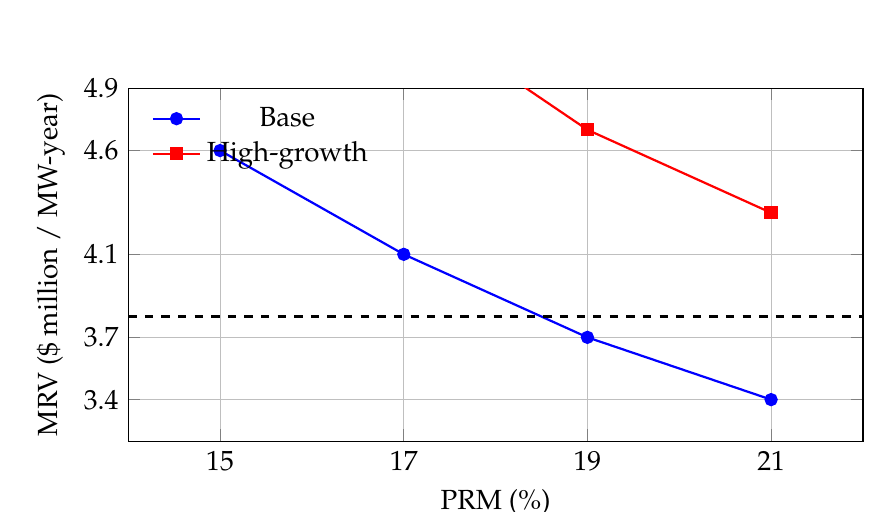
\begin{tikzpicture}
\begin{axis}[
  width=0.9\linewidth, height=0.5\linewidth,
  xlabel={PRM (\%)}, ylabel={MRV (\$~million / MW-year)},
  xmin=14, xmax=22, ymin=3.2, ymax=4.9,
  xtick={15,17,19,21}, ytick={3.4,3.7,4.1,4.6,4.9},
  grid=both, legend style={at={(0.02,0.98)},anchor=north west,draw=none,fill=none},
  every axis plot/.append style={thick}
]
% Base case
\addplot[blue,mark=*] coordinates {(15,4.6) (17,4.1) (19,3.7) (21,3.4)};
\addlegendentry{Base}

% High-growth (res +0.5\%)
\addplot[red,mark=square*] coordinates {(15,6.0) (17,5.3) (19,4.7) (21,4.3)};
\addlegendentry{High-growth}

% MC line
\addplot[dashed,black] coordinates {(14,3.8) (22,3.8)};
\node[anchor=west] at (axis cs:22,3.8) {$MC_{\text{cap}}=3.8$};

\end{axis}
\end{tikzpicture}
\caption{Marginal Reliability Value (MRV) as a function of Planning Reserve Margin (PRM). Dashed line shows marginal capacity cost; intersection gives economic PRM$^\star$.}
\end{figure}

\begin{figure}[h!]
\centering
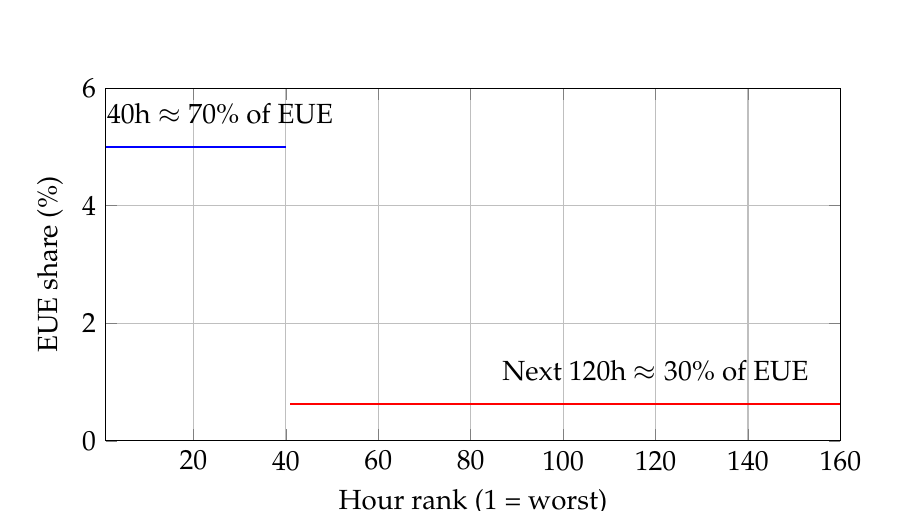
\begin{tikzpicture}
\begin{axis}[
  width=0.9\linewidth, height=0.5\linewidth,
  xlabel={Hour rank (1 = worst)}, ylabel={EUE share (\%)},
  xmin=1, xmax=160, ymin=0, ymax=6,
  grid=both, ymajorgrids=true,
  every axis plot/.append style={thick}
]
% Synthetic stack: first 40 hours high, next 120 moderate
\addplot[blue,domain=1:40,samples=40] {5};             % 5% per hour for 40 h -> 200%
\addplot[red,domain=41:160,samples=120] {0.625};       % 0.625% per hour for 120 h -> 75%
% normalize annotation
\node at (axis cs:20,5.5) {Top 40h $\approx 70\%$ of EUE};
\node at (axis cs:120,1.2) {Next 120h $\approx 30\%$ of EUE};
\end{axis}
\end{tikzpicture}
\caption{Illustrative concentration of EUE in top-risk hours.}
\end{figure}

\begin{figure}[h!]
\centering
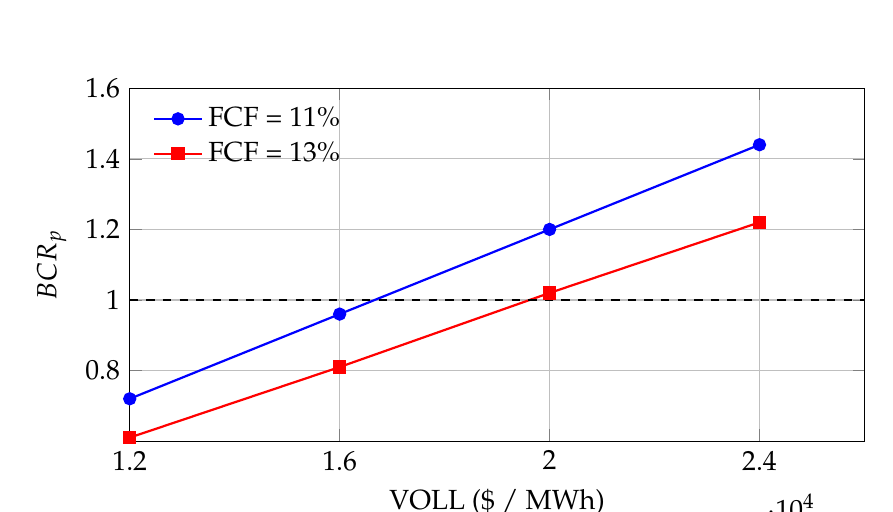
\begin{tikzpicture}
\begin{axis}[
  width=0.9\linewidth, height=0.5\linewidth,
  xlabel={VOLL (\$ / MWh)}, ylabel={$BCR_p$},
  xmin=12000, xmax=26000, ymin=0.6, ymax=1.6,
  xtick={12000,16000,20000,24000}, ytick={0.8,1.0,1.2,1.4,1.6},
  grid=both, legend style={at={(0.02,0.98)},anchor=north west,draw=none,fill=none},
  every axis plot/.append style={thick}
]
% BCR curve for fixed ΔEUE and Capex (base)
\addplot[blue,mark=*] coordinates {(12000,0.72) (16000,0.96) (20000,1.20) (24000,1.44)};
\addlegendentry{FCF = 11\%}

% Higher annualization (FCF 13\%)
\addplot[red,mark=square*] coordinates {(12000,0.61) (16000,0.81) (20000,1.02) (24000,1.22)};
\addlegendentry{FCF = 13\%}

% Reference BCR=1 line
\addplot[dashed,black] coordinates {(12000,1.0) (26000,1.0)};

\end{axis}
\end{tikzpicture}
\caption{Benefit–cost ratio $BCR_p$ as a function of VOLL and the fixed-charge factor (FCF).}
\end{figure}

\begin{table}[h!]
\centering
\caption{Worked Example Summary: Inputs, Intermediate Results, and Outputs (Zone $z$)}
\label{tab:worked_summary}
\renewcommand{\arraystretch}{1.15}
\begin{tabular}{llr}
\hline
\textbf{Item} & \textbf{Definition / Source} & \textbf{Value (Units)} \\
\hline
Baseline peak loads & $(L_{s,z,t_0}^{\text{peak}})$ by sector (A.13) & Res: 500; Com: 300; Ind: 200 (MW) \\
Growth rates & $(g_{\text{res}},g_{\text{com}},g_{\text{ind}})$ (A.13) & 1.5\%, 1.0\%, 0.5\% (/yr) \\
Growth volatility & $(\sigma_{s,z})$ (A.13) & 0.3\% (per annum) \\
Firm/VRE nameplate & $(C^{\text{firm}},C^{\text{VRE}})$ (A.13) & 900, 250 (MW) \\
Thermal FOR & $FOR$ (A.13) & 6\% \\
Import limit (base) & $I^{\max}$ (A.13) & 75 (MW) \\
Standardized VOLL & $VOLL_z$ (A.13) & 20{,}000 (\$/MWh) \\
\hline
Base EUE & $\widehat{EUE}_z^{\text{base}}$ (A.13) & 12{,}500 (MWh/yr) \\
Base RV & $\widehat{RV}_{\text{energy},z}^{\text{base}}$ (A.13) & 250 (M\$ / yr) \\
Finite-diff.\ MRV & $\widehat{MRV}_z$ (A.13) & 4.6 (M\$ / MW-yr) \\
MC of capacity & $MC_{cap,z}$ (A.13) & 3.8 (M\$ / MW-yr) \\
Economic PRM$^\star$ & $MRV=MC$; LOLE $\le$ target (A.13) & $\approx 19.3$ (\% above peak) \\
\hline
EUE (res +0.5\%) & $\widehat{EUE}_z^{\text{res}+0.5\%}$ (A.13) & 15{,}100 (MWh/yr) \\
MRV (res +0.5\%) & $\widehat{MRV}_z^{\text{res}+0.5\%}$ (A.13) & 6.0 (M\$ / MW-yr) \\
\hline
Transmission upgrade & $I^{\max}\!:\,75 \rightarrow 150$ (A.13) & $\Delta EUE=2{,}600$ (MWh/yr) \\
Annualized trans.\ cost & $Capex\times FCF$ (A.13) & 44 (M\$ / yr) \\
Benefit–cost ratio & $BCR=\Delta RV / \text{annualized cost}$ (A.13) & 1.18 (–) \\
\hline
Queue project (storage) & $100$ MW, 4 h; ELCC $=0.72$ (A.13) & Score $=2.83$ (M\$ / MW-yr) \\
\hline
\end{tabular}
\end{table}

\newpage

\section{Algorithmic Recipe: End-to-End Implementation (Pseudo-code)}
\label{sec:algo_recipe}

% Added 'breakable' to allow this box to flow across page boundaries
\begin{tcolorbox}[breakable, colback=lightgray, colframe=nousblue, title=\textsc{Algorithmic Recipe (UEVF--MRV with Demand Growth, Transmission Coupling, and Queue Scoring)}]

\noindent\textbf{Inputs (data and primitives).}
\begin{enumerate}
  \item Baseline sectoral load traces $L_{s,z,t_0}$ and sector/zone growth parameters $(g_{s,z},\sigma_{s,z})$.
  \item Resource and availability stack models $\tilde{C}^{avail}_{z,t}$ (forced outage rates, renewable profiles, maintenance, derates).
  \item Transmission representation (e.g., DC power flow / transfer limits / PTDF constraints) producing deliverable $C^{avail}_{z,t}$.
  \item Reliability valuation parameters: $\VOLL_z$; adequacy targets (e.g., $\LOLE_{target}$) and/or procurement price proxy $MC_{\mathrm{cap},z}$.\footnote{In the \textit{Refining MRV} paper, $MC$ is typically derived from the capacity demand curve (e.g., VRR/Net CONE constructs) and compared to MRV as a stop rule. Here we treat $MC_{\mathrm{cap},z}$ abstractly: it can be an observed market price, a planning shadow price, or an annualized VRR point. The key is unit alignment: USD/(MW$\cdot$yr) versus USD/MWh through $\VOLL$.}
  \item Simulation controls: number of synthetic years $N$, time granularity $\Delta t$ (hours), random seeds, and whether common random numbers (CRN) are used.\footnote{CRN means reusing the same underlying random draws when comparing $C_z$ vs. $C_z+\Delta C$ so the \emph{difference} in $EUE$ has lower variance. This is standard in reliability Monte Carlo when estimating small marginal effects.}
\end{enumerate}

\vspace{0.5em}
\noindent\textbf{Outputs (key objects).}
\begin{enumerate}
  \item Demand scenarios $\{L_{z,t}^{(\omega)}\}$ and reliability metrics $EUE_z$, $\LOLE_z$.
  \item Sensitivities $\partial EUE_z/\partial C_z$ and $\MRV_z$ (and optionally MRV-by-hour weights via $\alpha_t$).
  \item Calibrated $PRM^\star$ (or equivalently $C_z^\star$) satisfying economic optimality and any binding adequacy constraints.
  \item Transmission project screens $(\Delta EUE_z^{(p)}, \Delta RV^{(p)}_{\mathrm{energy}}, BCR_p)$.
  \item Queue prioritization scores $\mathrm{Score}_i$ (readiness/deliverability weighted) and a ranked shortlist.
\end{enumerate}

\vspace{0.8em}
\noindent\textbf{Procedure.}

\begin{enumerate}
  \item \textbf{Generate demand scenarios (sector $\rightarrow$ zonal aggregation).}
  For each scenario $\omega=1,\dots,N$ and for each $(s,z,t)$:
  \[
  L_{s,z,t}^{(\omega)} = L_{s,z,t_0}\cdot \exp\!\Big((g_{s,z}+\epsilon^{(\omega)}_{s,z})(t-t_0)\Big),
  \qquad \epsilon^{(\omega)}_{s,z}\sim\mathcal{N}(0,\sigma_{s,z}^2).
  \]
  Aggregate to zone load:
  \[
  L_{z,t}^{(\omega)}=\sum_s L_{s,z,t}^{(\omega)}.
  \]
  \footnote{If you have hourly shape forecasts (e.g., electrification load shapes, data center ramp profiles, or weather-conditioned demand), inject them here as multiplicative or additive shape factors rather than baking them into $\epsilon_{s,z}$. Keep $g_{s,z}$ as the long-run drift and use scenario overlays for intra-annual dynamics. This is also the clean bridge to the \textit{Demand Projection Integration} note you referenced as a companion document.}

  \item \textbf{Simulate available capacity with outages, renewables, and deliverability.}
  For each scenario-year $\omega$ and hour $t$, sample:
  \begin{itemize}
    \item forced outages / derates $\Rightarrow$ thermal availability,
    \item renewable generation (or net-load) uncertainty,
    \item transmission deliverability / import constraints.
  \end{itemize}
  Produce a deliverable availability trajectory $C^{avail,(\omega)}_{z,t}$.

  \footnote{The clean UEVF decomposition is: (i) create an \emph{unconstrained} available stack $\tilde{C}^{avail}_{z,t}$ (outages, renewables, maintenance), then (ii) apply a deliverability operator (PTDF/transfer limits, local constraints) to obtain $C^{avail}_{z,t}$. This is exactly where the \textit{Refining MRV} paper’s “locationalization” work lives: scarcity is pocketed, and deliverability is the gatekeeper.}

  \item \textbf{Compute shortages and reliability metrics.}
  For each $\omega$ and $t$:
  \[
  S_{z,t}^{(\omega)}=\max\{0,\;L_{z,t}^{(\omega)}-C^{avail,(\omega)}_{z,t}\}.
  \]
  Estimate:
  \[
  \widehat{EUE}_z=\frac{1}{N}\sum_{\omega=1}^N \sum_{t\in T} S_{z,t}^{(\omega)}\,\Delta t,
  \qquad
  \widehat{LOLE}_z=\frac{1}{N}\sum_{\omega=1}^N \sum_{t\in T}\mathbb{1}\{S_{z,t}^{(\omega)}>0\}\,\Delta t.
  \]
  \footnote{Be explicit about whether $\LOLE$ is reported in hours/year or days/year; many planning documents use days/year, while hourly Monte Carlo naturally yields hours/year. Conversion is mechanical but mix-ups are common.}

  \item \textbf{Estimate $\partial EUE_z/\partial C_z$ and MRV (finite difference with CRN).}
  Choose a small increment $\Delta C$ (e.g., $0.5$--$2$ MW) and re-evaluate $EUE_z$ with $C_z+\Delta C$ added to the deliverable stack (holding the random draws fixed if using CRN):
  \[
  \widehat{\frac{\partial EUE_z}{\partial C_z}}
  \approx
  \frac{\widehat{EUE}_z(C_z+\Delta C)-\widehat{EUE}_z(C_z)}{\Delta C}.
  \]
  Then compute
  \[
  \widehat{MRV}_z
  =
  -\,\VOLL_z\cdot \widehat{\frac{\partial EUE_z}{\partial C_z}}.
  \]
  \footnote{Two practical rules: (i) pick $\Delta C$ large enough that the signal is above Monte Carlo noise, small enough to approximate a derivative; (ii) if you see sign instability across seeds, increase $N$ or use CRN. In the \textit{Refining MRV} paper, this derivative is what makes MRV a \emph{marginal procurement signal} rather than a static reliability metric.}

  \item \textbf{Calibrate $PRM^\star$ (economic optimum with adequacy backstop).}
  Solve for the reserve margin (or equivalent capacity level) that equalizes marginal cost and marginal reliability value:
  \[
  PRM^\star \;\in\; \arg\min_{PRM}\; \big|\widehat{MRV}_z(PRM)-MC_{\mathrm{cap},z}\big|
  \quad\text{s.t.}\quad \widehat{LOLE}_z(PRM)\le \LOLE_{target}.
  \]
  \footnote{This is the “MRV = MC” condition proven in the PRM optimality section. In practice you often hit the LOLE constraint first in tight systems; treat the constraint as a hard floor (engineering requirement) and the MRV=MC as the interior economic optimum when slack exists.}

  \item \textbf{Transmission screen (project-level reliability benefit).}
  For each candidate transmission project $p$ (new line, reconductoring, transformer, topology action):
  \begin{enumerate}
    \item Modify the deliverability/transfer limits $\Rightarrow C^{avail,(p)}_{z,t}$.
    \item Recompute $\widehat{EUE}^{(p)}_z$ using the same demand/outage draws (CRN).
    \item Compute
    \[
    \Delta \widehat{EUE}^{(p)}_z = \widehat{EUE}^{base}_z-\widehat{EUE}^{(p)}_z,
    \qquad
    \Delta \widehat{RV}^{(p)}_{\mathrm{energy}}=\Delta \widehat{EUE}^{(p)}_z\cdot \VOLL_z,
    \qquad
    BCR_p=\frac{\Delta \widehat{RV}^{(p)}_{\mathrm{energy}}}{Capex_{\mathrm{trans},p}}.
    \]
  \end{enumerate}
  \footnote{If you want to align fully with the \textit{Refining MRV} paper’s philosophy, treat GETs/topology actions as “transmission projects” here and score them identically. The point is to compare MW of deliverability unlocked to the monetized scarcity reduction it produces.}

  \item \textbf{Interconnection queue scoring (reliability-value prioritization).}
  For each generation/storage project $i$ interconnecting in zone $z$:
  \[
  \mathrm{Score}_i
  =
  \widehat{MRV}_z \cdot ELCC_i \cdot w_{\mathrm{readiness},i}\cdot w_{\mathrm{deliverability},i}.
  \]
  Rank descending $\mathrm{Score}_i$, then apply feasibility constraints (cluster upgrade coordination, deliverability caps, CRZ/LDA limits).\footnote{“CRZ/cluster” constraints here mean the institutional realities that you can’t pick projects independently: study clusters share upgrades, deliverability is pocketed, and transmission constraints create coupling. This is exactly why a scalar score is used for \emph{ordering} and \emph{screening}, not as a full substitute for joint optimization. The \textit{Refining MRV} paper’s co-optimization refinement is the next step when you want portfolio-optimal picks rather than ranked lists.}
\end{enumerate}
\end{tcolorbox}

\end{document}
